% -*- Mode:TeX -*-

%% IMPORTANT: The official thesis specifications are available at:
%%            https://sites.google.com/a/ncf.edu/thesis/Thesis-Guidelines?pli=1
%%
%%            Please verify your thesis' formatting and copyright
%%            assignment before submission.

%% The documentclass options along with the pagestyle can be used to generate
%% a technical report, a draft copy, or a regular thesis.  You may need to
%% re-specify the pagestyle after you \include  cover.tex.  For more
%% information, see the first few lines of mitthesis.cls. 

%\documentclass[12pt,vi,twoside]{ncfthesis}
%%
%%  If you want your thesis copyright to you instead of NCF, use the
%%  ``vi'' option, as above.
%%
%\documentclass[12pt,twoside,leftblank]{ncfthesis}
%%
%% If you want blank pages before new chapters to be labelled ``This
%% Page Intentionally Left Blank'', use the ``leftblank'' option, as
%% above. 

\documentclass[12pt, doublespace]{ncfthesis}
\usepackage{lgrind}
\usepackage[fleqn]{mathtools}
\usepackage{amsmath}
\usepackage{amssymb} % for math symbols such as \therefore
\usepackage{amsthm}
\newtheorem{theorem}{Theorem}[section]
%\newtheorem{corollary}{Corollary}[theorem]
\newtheorem{lemma}[theorem]{Lemma}
\newtheorem{remark}{Remark}

\usepackage{algorithm}
\usepackage{algpseudocode}
\usepackage{graphicx} % package to manage images
\usepackage{subcaption} % package for subfigures
\graphicspath{ {figures/} }
\usepackage{wrapfig}
\usepackage{listings} %code extracts
\usepackage{xcolor} %custom colours
\usepackage{mdframed} %nice frames
\usepackage{multicol} % for tables
\usepackage{multirow} % for tables
\usepackage{makecell} % for tables
\usepackage{diagbox} % for tables
\usepackage{xcolor,colortbl} % for coloring tables


\definecolor{light-gray}{gray}{0.95} %the shade of grey that stack exchange uses

\usepackage[backend=biber]{biblatex}
\addbibresource{mainBib.bib}

\setcounter{biburlnumpenalty}{100}
\setcounter{biburlucpenalty}{100}
\setcounter{biburllcpenalty}{100} 

\usepackage{url}
%% These have been added at the request of the MIT Libraries, because
%% some PDF conversions mess up the ligatures.  -LB, 1/22/2014
\usepackage{cmap}
\usepackage[T1]{fontenc}
\pagestyle{plain}



\begin{document}
% -*-latex-*-
% 
% For questions, comments, concerns or complaints:
% thesis@mit.edu
% 
%
% $Log: cover.tex,v $
% Revision 1.8  2008/05/13 15:02:15  jdreed
% Degree month is June, not May.  Added note about prevdegrees.
% Arthur Smith's title updated
%
% Revision 1.7  2001/02/08 18:53:16  boojum
% changed some \newpages to \cleardoublepages
%
% Revision 1.6  1999/10/21 14:49:31  boojum
% changed comment referring to documentstyle
%
% Revision 1.5  1999/10/21 14:39:04  boojum
% *** empty log message ***
%
% Revision 1.4  1997/04/18  17:54:10  othomas
% added page numbers on abstract and cover, and made 1 abstract
% page the default rather than 2.  (anne hunter tells me this
% is the new institute standard.)
%
% Revision 1.4  1997/04/18  17:54:10  othomas
% added page numbers on abstract and cover, and made 1 abstract
% page the default rather than 2.  (anne hunter tells me this
% is the new institute standard.)
%
% Revision 1.3  93/05/17  17:06:29  starflt
% Added acknowledgements section (suggested by tompalka)
% 
% Revision 1.2  92/04/22  13:13:13  epeisach
% Fixes for 1991 course 6 requirements
% Phrase "and to grant others the right to do so" has been added to 
% permission clause
% Second copy of abstract is not counted as separate pages so numbering works
% out
% 
% Revision 1.1  92/04/22  13:08:20  epeisach

% NOTE:
% These templates make an effort to conform to the NCF Thesis specifications,
% however the specifications can change.  We recommend that you verify the
% layout of your title page with your thesis advisor and/or the NCF 
% Library before printing your final copy.
\title{State Estimation of an Unmanned Ground Vehicle Using Inexpensive Sensors}

\author{Noah Johnson}

\division{Division of Natural Sciences}

% If the thesis is for two degrees simultaneously, list them both
% separated by \and like this:
% \degree{Doctor of Philosophy \and Master of Science}
\degree{Bachelor of Arts in Computer Science \and Bachelor of Arts in Applied Mathematics}

\degreemonth{May}
\degreeyear{2017}
\thesisdate{May 18, 2017}

% If there is more than one thesis sponsor,
% you'll have to go modify the ncfthesis.cls file (under \endabstractpage

\sponsor{Professor Gary Kalmanovich}

% Make the titlepage based on the above information.  If you need
% something special and can't use the standard form, you can specify
% the exact text of the titlepage yourself.  Put it in a titlepage
% environment and leave blank lines where you want vertical space.
% The spaces will be adjusted to fill the entire page.  The dotted
% lines for the signatures are made with the \signature command.
\maketitle




%%%%%%%%%%%%%%%%%%%%%%%%%%%%%%%%%%%%%%%%%%%%%%%%%%%%%%%%%%%%%%%%%%%%%%
% -*-latex-*-


\pagenumbering{roman}
\setcounter{page}{2}

\section*{Acknowledgments}

This is the acknowledgements section.  You should replace this with your
own acknowledgements.
  % -*- Mode:TeX -*-
%% This file simply contains the commands that actually generate the table of
%% contents and lists of figures and tables.  You can omit any or all of
%% these files by simply taking out the appropriate command.  For more
%% information on these files, see appendix C.3.3 of the LaTeX manual. 
\tableofcontents
\newpage
\listoffigures
\newpage
\listoftables

%% The text of your abstract and nothing else (other than comments) goes here.
%% It will be single-spaced and the rest of the text that is supposed to go on
%% the abstract page will be generated by the abstractpage environment.
\begin{abstractpage}
Autonomous navigation is an important emerging technology with applications in warehouse automation, shipping, and  personal navigation. Hands on experimentation often proves too expensive for individuals at the undergraduate level, with common research platform costing several thousand dollars. In this thesis, I present a design for a cheap ground vehicle capable of fusing sensor data into a local state estimate. Costs were minimized by using personal components owned by most students, namely a personal laptop and smartphone. This should be an effective base for research into autonomous navigation.
\end{abstractpage}

\pagenumbering{arabic}
\chapter*{Introduction}

%Goal
This rover 
Create a cheap outdoors autonomous robot. Given a 'map' of the New College campus, this robot should be able to navigate from one outdoors location to another using footpaths. In doing so, it should dynamically avoid obstacles such as people, and recalculate alternate routes when a route is unexpectedly blocked.

%navigation
intro to the concept of navigation

Since a map with GPS coordinates is provided, this is not Simultaneous Localization and Mapping (SLAM), but a simplified navigation problem. 

% design
The rover base consists of a Lynxmotion rover, an Arduino, and a Sabertooth motor driver. Sensors available include two quadrature rotary encoders, a mobile phone, and an ultrasonic distance sensor. The Arduino acts as a low-level robotic controller, publishing wheel encoder and range data, and accepting motor velocity commands. An Android app publishes IMU and GPS data from the mobile phone, and the laptop fuses these readings into a state estimation of pose and velocity using an extended Kalman filter.

%Choice of Sensors
IR, Microsoft Kinect
can't use because the rover will be outdoors during the day and the sun gives off ambient IR radiation.

LIDAR - state of the art

And LIDAR sensors would be too costly. constrained by cheap hardware, and the inability to use IR or LIDAR sensors.

%Thesis Structure
The rest of this thesis is organized as follows.

Chapter 2 covers the probability theory behind the extended kalman filter, which is an iterative update algorithm used to fuse noisy sensor data into a local state estimate for the rover. It may be skipped if one is not interested in the mathematical details.

Chapter 3 describes the hardware components used in this project, their electrical connections, and the general design.

Chapter 4 continues the description of physical connections with respect to the Arduino circuit board, and also describes the software which runs on that board and how it interfaces with the rest of the system.

Chapter 5 gives a brief overview of the Robot Operating System (ROS), and how it's used in this project. It then meanders through every software process used, and how they communicate through ROS.

Chapter 6 describes the results of an experimental test conducted with the rover. Limitations of and extensions to the current design are also mentioned.

\addcontentsline{toc}{chapter}{Introduction}
\newcommand{\bel}{\mathrm{bel}}

\chapter{Theory}

This chapter will dive into the mathematical theory behind the recursive state estimator used in this project, the Extended Kalman Filter. Steps have been taken to carefully explain every computation made for the less mathematically inclined. This section is largely based on chapters 1-3 of the book Probabilistic Robotics \cite{probabilisticRobotics}, which the interested reader should view for a broader look at the same material. 

\section{Probability Theory Background} \label{sectionProbTheory}
To gather information about their environment, robots use sensor data. This data always has some amount of random noise associated with it. Thus probability theory is vital to creating models which incorporate  this uncertainty. Here we will review some probability theory results which will be needed in this chapter.

% technically p(X=x) = 0 for continuous PDFs, but we're working with finite precision computers so who cares. It's easier to think of this way.
Random variables are objects from which specific numbers may be observed. Let X be a continuous random variable - that is, observations of X are real numbers. We will represent the probability of observing any particular real number x from X as \( p(X = x) \equiv p(x)\). This defines a function \(p: \mathbb{R} \to \mathbb{R}\) representing the distribution of probabilities across the real numbers. Throughout this chapter, we will refer to such functions as Probability Density Functions (PDFs). Note the basic result that for every PDF \(p\) constructed from a random variable X, \(\int p(x)dx = 1\), which is to say that the observed value from X will be some real number with 100\% certainty.

An important tool for describing PDFs is their expectation. \(E[X]\) is the expected value or mean of X. Note that the expectation operator is linear: \(E[\alpha X + \beta Y] = \alpha E[X] + \beta E[Y]\).

For two random variables X and Y, we will define their covariance to be
\[
cov(X,Y) = E[(X - E[X])(Y - E[Y])]
\] This gives a measure of the co-dependence between X and Y.

The same concepts may be scaled up to random vectors, which are \(n\)-dimensional collections of random variables. Then \(X = (X_1,X_2,...,X_n)^T\), and \(p:\mathbb{R}^n \to \mathbb{R}\) still defines a PDF. The expectation becomes \[
E[X] = \begin{pmatrix}
E[X_1] \\
\vdots \\
E[X_n]
\end{pmatrix} 
\]

and we can define a covariance matrix \(\Sigma\) for the random vector:
\[
\Sigma = E[(X - E[X])(X - E[X])^T] = \begin{pmatrix}
cov(X_1,X_1)  \dots cov(X_1,X_n) \\
\vdots \ddots \vdots \\
cov(X_n,X_1)  \dots cov(X_n,X_n)
\end{pmatrix} 
\]


Now consider three random variables: X, Y, and Z. Define their joint distribution \(p(X=x\ \textrm{and}\ Y=y\ \textrm{and}\ Z=z) \equiv p(x,y,z)\), and the conditional probability \(p(X=x\ \textrm{given that}\ Y=y\ \textrm{and}\ Z=z) \equiv p(x \mathbin{\vert} y,z)\). The conditional probability is given to be
\begin{equation} \label{eqCondProb}
p(x \mathbin{\vert} y,z) = \frac{p(x,y,z)}{p(y,z)}
\end{equation}

The \textit{Law of Total Probability} states that \(p(x) = \int p(x,y)dy\). Conditioning this law on a third random variable Z, and incorporating the definition of conditional probability (Eq. \ref{eqCondProb}), we end up with the following version of this law:
\begin{multline} \label{eqTotalProb}
p(x \mathbin{\vert} z) = \int p(x,y \mathbin{\vert} z)dy = \int \frac{p(x,y,z)}{p(z)}  \\
= \int \frac{p(x,y,z)}{p(y,z)} * \frac{p(y,z)}{p(z)} = \int p(x \mathbin{\vert} y,z) p(y\mathbin{\vert}z)dy \hfill
\end{multline}

In a similar fashion, we can use the definition of conditional probability (Eq. \ref{eqCondProb}) to derive a version of Bayes' Rule. 
\begin{multline} \label{eqBayesThm}
p(x \mathbin{\vert} y,z) = \frac{p(x,y,z)}{p(y,z)} = \frac{p(y,x,z)}{p(x,z)} * \frac{p(x,z)}{p(z)} * \frac{p(z)}{p(y,z)} \\
= \frac{p(y \mathbin{\vert} x,z)p(x\mathbin{\vert}z)}{p(y \mathbin{\vert} z)} \hfill
\end{multline}
In the future these will prove to be useful tools to update a PDF with new information. When presented with new information that  \(Y = y\), one may use Bayes' Rule to transform the current PDF \(p(x \mathbin{\vert}z)\) into the new posterior PDF \(p(x \mathbin{\vert} y,z)\). %from the inverse conditional probability \(p(y \mathbin{\vert} x)\) and the prior PDF \(p(x)\).

\section{Bayes Filter}
\subsection{Scenario}
Now, back to the inner workings of our rover. Consider the general case of a robot which uses some array of sensors to gather information about its environment. The robot wishes to use these measurements to estimate its current state, where the state is a collection of variables of interest (e.g. position, orientation, velocity, acceleration, etc.).

For simplicity, let us consider the rover to operate in discrete time steps (\(t=0,1,2,...\)). We can encode all state variables of interest in the vector \(x_t = (x_{1_t}, x_{2_t}, ... , x_{n_t})^T\). Similarly, let \(z_t = (z_{1_t}, z_{2_t}, ... , z_{k_t})^T\) represent a sensor measurement at time \(t\). For both of these vectors we will use the compact notation \(a_{1:t} = a_1, a_2, ..., a_t\) to denote the set of all vectors up to and including time \(t\).

The robot wishes to know \(x_t\), however this true state is hidden. It only has access to raw sensor data in the form of \(z_{1:t}\). Sensor measurements always contain some level of noise due to ambient interference, no matter how precise the hardware. Thus each of these measurements will have some amount of error, and the robot will need to account for this in its state estimate. The robot can do this by constructing a PDF assigning a probability to every possible realization of \(x_t\). This PDF will represent the robot's belief in its current state, and should be conditioned on all available data. Thus we will define the robot's belief distribution to be:
\begin{equation} \label{eqBel}
\bel(x_t) = p(x_t \mathbin{\vert} z_{1:t})
\end{equation}

\subsection{Derivation}
Now we must figure out how to compute \(\bel(x_t)\). Let us start by using Bayes' Rule to rewrite \(\bel(x_t)\):
\begin{equation*}
\bel(x_t) = p(x_t \mathbin{\vert} z_{1:t}) = p(x_t \mathbin{\vert} z_t, z_{1:t-1}) = \frac{p(z_t \mathbin{\vert} x_t, z_{1:t-1})p(x_t \mathbin{\vert} z_{1:t-1})}{p(z_t \mathbin{\vert} z_{1:t-1})}
\end{equation*}

In order to continue, we will need to simplify \(p(z_t \mathbin{\vert} x_t, z_{1:t-1})\). Here we will make an important assumption. We will assume that the state \(x_t\) satisfies the Markov property: that is, \(x_t\) perfectly encapsulates all current and prior information \cite{robot_localization_paper}. Thus if \(x_t\) is known, then \(z_{1:t}\) are redundant, i.e. \(p(z_t \mathbin{\vert} x_t, z_{1:t}) = p(z_t \mathbin{\vert} x_t)\).

This assumption lets us remove consideration of past sensor measurements, and to rewrite the belief distribution as:
\begin{equation*}
\bel(x_t) = \frac{p(z_t \mathbin{\vert} x_t)p(x_t \mathbin{\vert} z_{1:t-1})}{p(z_t \mathbin{\vert} z_{1:t-1})}
\end{equation*}

Notice that \(p(z_t \mathbin{\vert} z_{1:t-1})\) is a constant with respect to \(x_t\). Thus it makes sense to define \(\eta = (p(z_t \mathbin{\vert} z_{1:t-1}))^{-1}\) and rewrite the belief distribution as:
\begin{equation*}
\bel(x_t) = \eta p(z_t \mathbin{\vert} x_t) p(x_t \mathbin{\vert} z_{1:t-1})
\end{equation*}
Notice that \(\bel(x_t)\) is a PDF, so it must integrate to 1. \(\eta\) acts as a normalizing constant enforcing this constraint.

Now \(\bel(x_t)\) has been split into two distributions of interest. Looking closely one may notice that \(p(x_t \mathbin{\vert} z_{1:t-1})\) is simply our original belief distribution, Eq. \ref{eqBel}, but not conditioned on the most recent sensor measurement \(z_t\). Let us refer to this distribution as \(\overline{\bel}(x_t)\), and break it down further using the \textit{Law of Total Probability} (Eq. \ref{eqTotalProb}) and our Markov assumption:
\begin{multline*}
\overline{\bel}(x_t) = p(x_t \mathbin{\vert} z_{1:t-1}) \\
= \int p(x_t \mathbin{\vert} x_{t-1}, z_{1:t-1}) p(x_{t-1} \mathbin{\vert} z_{1:t-1})dx_{t-1} \hfill \text{(by Eq. \ref{eqTotalProb})}\\
= \int p(x_t \mathbin{\vert} x_{t-1}) p(x_{t-1} \mathbin{\vert} z_{1:t-1})dx_{t-1} \hfill \text{  (by Markov assumption)} \\
= \int p(x_t \mathbin{\vert} x_{t-1}) \bel(x_{t-1})dx_{t-1}  \hfill \text{(by Eq. \ref{eqBel})}
\end{multline*}

We have arrived at a recursive definition of \(\bel(x_t)\) with respect to \(\bel(x_{t-1})\)! As long as \(p(x_t \mathbin{\vert} x_{t-1})\) and \(p(z_t \mathbin{\vert} x_t)\) are known, we can recursively calculate \(\bel(x_t)\) from some starting belief \(\bel(x_0)\).

\(p(x_t \mathbin{\vert} x_{t-1})\) defines a stochastic model for the robot's state, determining how the robot's state will evolve over time. This PDF will be referred to as the \textit{state transition probability}  \cite{probabilisticRobotics}.

\(p(z_t \mathbin{\vert} x_t)\) also defines a stochastic model, modeling the sensor measurements \(z_t\) as noisy projections of the robot's state. This PDF will be referred to as the \textit{measurement probability}  \cite{probabilisticRobotics}.

Once we assume the \textit{state transition probability} and \textit{measurement probability} PDFs are known, we can finally construct the algorithm known as Bayes' Filter:

\begin{algorithm} 
\caption{Bayes Filter} 
\label{alg:BayesFilter}
\begin{algorithmic}[1]
\Function{BayesFilterIterate}{ $\bel(x_{t-1})$, $z_t$ }
	\State{\(\overline{\bel}(x_t) = \int p(x_t \mathbin{\vert} x_{t-1}) \bel(x_{t-1})dx_{t-1} \)}
	\State{\(\bel(x_t) = \eta p(z_t \mathbin{\vert} x_t) \overline{\bel}(x_t) \)}
	\State{Set \(\int \bel(x_t)dx_t = 1\), and solve for \(\eta \)}
	\State{Use \(\eta\) to normalize \(\bel(x_t)\)}
	\State \Return{\(\bel(x_t)\)}
	\EndFunction
\end{algorithmic}
\end{algorithm}

%\subsection{Example}
\section{Extended Kalman Filter} \label{sectionEKF}

The most widely used algorithm implementing Bayes Filter is the Extended Kalman Filter (EKF). This filter approximates the PDFs found in Bayes Filter with multi-variate normal distributions. This class of PDFs are unimodal, and have the form 
\begin{equation} \label{eqDefNormal}
p(x) = N(x; E[X],\Sigma) = det(2 \pi \Sigma)^{-\frac{1}{2}} * exp \{-\frac{1}{2} (x - E[X])^T \Sigma^{-1} (x - E[X])\}
\end{equation}
where \(E[X]\) and \(\Sigma\) are the mean and covariance matrix of the random vector X, as described in section \ref{sectionProbTheory}. Notice that the mean and covariance matrix are sufficient to uniquely define any particular normal  distribution, and so the EKF only needs to keep track of a vector and matrix per PDF. So the belief distribution can be totally described by the best estimate for the state vector and the uncertainty in that estimate:
\begin{equation} \label{eqBelNormalDef}
\bel(x_t) = N(x_t; \mu_t,\Sigma_t)
\end{equation}
where \(\mu_t = E[X_t]\) is the mean or best state estimate, and \(\Sigma_t\) is the covariance matrix or uncertainty. These are the values which our new algorithm will try to compute; doing so will completely describe \(\bel(x_t)\).

Recall that Algorithm \ref{alg:BayesFilter} (Bayes' Filter) requires that the state transition PDF \(p(x_t \mathbin{\vert} x_{t-1})\) be given. So let us assume that the evolution of state is known via some model \[X_t =  g(X_{t-1}) + \epsilon_t\] where \(g: \mathbb{R}^n \to \mathbb{R}^n\) is some arbitrary function defining how the state evolves, and \(\epsilon_t\) is additive noise in the model. We will define \(\epsilon_t\) to be a random vector of normal distribution with mean 0 and covariance matrix \(R_t\).

% Why must we linearize?
%In order to
If \(g\) is nonlinear, then it will distort the prior belief such that the posterior belief will no longer be normally distributed. In order to maintain our normal distribution assumption, we will have to make an approximation to the model. We will do so by linearizing this model using a first-order Taylor series approximation around the current best estimate, \(\mu_{t-1}\).
\begin{multline*}
g(X_{t-1}) \approx g(\mu_{t-1}) + \frac{\partial g(\mu_{t-1})}{\partial X_{t-1}} (X_{t-1} - \mu_{t-1}) \\
= g(\mu_{t-1}) + G_t (X_{t-1} - \mu_{t-1}) \hfill
\end{multline*}
where \[
G_t = \begin{bmatrix} 
\frac{\partial g_1(\mu_{t-1})}{\partial X_{1_{t-1}}} & \dots & \frac{\partial g_1(\mu_{t-1})}{\partial X_{n_{t-1}}}\\
\vdots & \ddots & \vdots & \\
\frac{\partial g_n(\mu_{t-1})}{\partial X_{1_{t-1}}} & \dots & \frac{\partial g_n(\mu_{t-1})}{\partial X_{n_{t-1}}} 
\end{bmatrix} \] is the Jacobian of \(g\) evaluated at \(\mu_{t-1}\). Then our approximate model is given by
\begin{equation*}
X_t \approx g(\mu_{t-1}) + G_t (X_{t-1} - \mu_{t-1}) + \epsilon_t
\end{equation*}
To describe the state transition PDF \(p(x_t \mathbin{\vert} x_{t-1})\), we are interested in finding its expectation and covariance matrix. Because its PDF is conditioned on \(x_{t-1}\), we likewise will condition its expectation. Then we can calculate the mean:
\begin{multline*}
E[X_t\ \mathbin{\vert} X_{t-1}] \approx E[g(\mu_{t-1}) + G_t (X_{t-1} - \mu_{t-1}) + \epsilon_t\ \mathbin{\vert} X_{t-1}] \\
= E[g(\mu_{t-1}) + G_t (X_{t-1} - \mu_{t-1})\ \mathbin{\vert} X_{t-1}] + E[\epsilon_t\ \mathbin{\vert} X_{t-1}] \hfill \text{(by linearity of E[X])} \\
= E[g(\mu_{t-1}) + G_t (X_{t-1} - \mu_{t-1})\ \mathbin{\vert} X_{t-1}] \hfill \text{(by the definition of \(\epsilon_t\))} \\
= g(\mu_{t-1}) + G_t (X_{t-1} - \mu_{t-1}) \hfill
\end{multline*}
and the covariance matrix:
\begin{multline*}
E[(X_t - E[X_t])(X_t - E[X_t])^T\ \mathbin{\vert} X_{t-1}] \\ \approx E[(g(\mu_{t-1}) + G_t (X_{t-1} - \mu_{t-1}) + \epsilon_t - g(\mu_{t-1}) - G_t (X_{t-1} - \mu_{t-1})) \\
* (g(\mu_{t-1}) + G_t (X_{t-1} - \mu_{t-1}) + \epsilon_t - g(\mu_{t-1}) - G_t (X_{t-1} - \mu_{t-1}))^T\ \mathbin{\vert} X_{t-1}] \\
= E[\epsilon_t \epsilon_t^T\ \mathbin{\vert} X_{t-1}] = E[(\epsilon_t - 0)(\epsilon_t - 0)^T\ \mathbin{\vert} X_{t-1}] \\
= E[(\epsilon_t - E[\epsilon_t\ \mathbin{\vert} X_{t-1}])(\epsilon_t - E[\epsilon_t\ \mathbin{\vert} X_{t-1}])^T\ \mathbin{\vert} X_{t-1}] \\
= R_t \hfill \text{(by the definition of \(\epsilon_t\))} \end{multline*}
and so its Gaussian distribution is approximately
\begin{equation} \label{eqStateTransitionNormalDef}
p(x_t \mathbin{\vert} x_{t-1}) \approx N(x_t;g(\mu_{t-1}) + G_t (x_{t-1} - \mu_{t-1}),R_t)
\end{equation}

\subsection{Matrix Calculus}
% talk about matrix calculus and vector differentiation. (AB)^T = B^T A^T, (A+B)^T = A^T + B^T, if A is symmetric then so is A^-1, lemmas etc.
For the mathematical derivation of the EKF which lies ahead, we will be working with matrix calculus.

For the benefit of the unfamiliar reader, here we will restate some elementary results which will be needed to follow along.

For \(A,B \in \mathbb{R}^{nxn}\):
\begin{gather}
A = \begin{pmatrix}
A_{11}  \dots A_{1n} \\
\vdots  \ddots  \vdots \\
A_{n1} \dots  A_{nn}
\end{pmatrix}  \implies A^T = \begin{pmatrix}
A_{11}  \dots A_{n1} \\
\vdots  \ddots  \vdots  \\
A_{1n} \dots A_{nn}
\end{pmatrix} \\
(AB)^T = B^T A^T \\
(A+B)^T = A^T + B^T \\
A \text{ is symmetric} \implies A^T = A \\
A \text{ is symmetric } \implies A^{-1} \text{ is symmetric } 
\end{gather}

\begin{lemma} \label{lemma1}
	For \(x \in \mathbb{R} ^n \) and \(A \in \mathbb{R}^{nxn}\), A symmetric,
	\[\frac{\partial (x^T A x)}{\partial x} = 2 A x\]
\end{lemma}
\begin{proof}
	\begin{multline*}
	\text{Define } f: \mathbb{R}^n \to \mathbb{R}, f(x) = x^T A x \\
	x = \begin{pmatrix}
	x_1 \\
	\vdots \\
	x_n
	\end{pmatrix} \text{, }
	\frac{\partial{f}}{\partial{x}} = 
	\begin{pmatrix}
	\frac{\partial{f}}{\partial{x_1}} \\
	\vdots \\
	\frac{\partial{f}}{\partial{x_n}}
	\end{pmatrix} \text{, } e_i = 
	\begin{pmatrix}
	0 \\
	\vdots \\
	1 \\
	\vdots \\
	0
	\end{pmatrix} \\
	\text{For } h \in \mathbb{R} \text{,} \\
	\frac{\partial f}{\partial x_i} = \lim_{h \rightarrow 0} \frac{f(x+h e_i) - f(x)}{h} = \lim_{h \rightarrow 0} \frac{(x + h e_i)^T A (x + h e_i) - x^T A x}{h} \\
	= \lim_{h \rightarrow 0} \frac{ x^T A x + h * x^T A e_i + h * e_i^T A x + h^2 * e_i^T A e_i - x^T A x}{h} \\
	= \lim_{h \rightarrow 0} \frac{ h [x^T A e_i + e_i^T A x + h * e_i^T A e_i]}{h} = \lim_{h \rightarrow 0} ( x^T A e_i + e_i^T A x + h * e_i^T A e_i) \\
	= x^T A e_i + e_i^T A x = e_i^T A^T x + e_i^T A x \hfill \text{(\(x^T A e_i\) is 1x1 \(\therefore x^T A e_i\) is symmetric)} \\
	= e_i^T ( A^T + A) x  = e_i^T ( A + A) x = e_i^T (2A x) \hfill \text{(by symmetry of A)} \\
	\text{Which tells us that the \(i^{th}\) component of \(\frac{\partial f}{\partial x} \) is equal to the \(i^{th}\) component of \(2Ax\).} \\
	\therefore \frac{\partial f}{\partial x} = 2Ax \hfill
	\end{multline*}
\end{proof}

\begin{lemma} \label{lemma2}
	For \(x,a \in \mathbb{R}^n \),
	\(\frac{\partial (x^T a)}{\partial x} = \frac{\partial (a^T x)}{\partial x} = a\)  
\end{lemma}
\begin{proof}
	\begin{multline*}
	\frac{\partial (a^T x)}{\partial x}  = \begin{pmatrix}
	\frac{\partial (a^T x)}{\partial x_1} \\
	\vdots \\
	\frac{\partial (A^T x)}{\partial x_n}
	\end{pmatrix} = \begin{pmatrix}
	\frac{\partial (a_1 x_1 + \dots + a_n x_n)}{\partial x_1} \\
	\vdots \\
	\frac{\partial (a_1 x_1 + \dots + a_n x_n)}{\partial x_n}
	\end{pmatrix}
	= \begin{pmatrix}
	a_1 \\
	\vdots \\
	a_n
	\end{pmatrix}
	= a \\
	a^T x \text{ has dimension 1 by 1, } \therefore a^T x = (a^T x)^T = x^T a \\
	\implies \frac{\partial (a^T x)}{\partial x} = \frac{\partial (x^T a)}{\partial x} = a \hfill
	\end{multline*}
\end{proof}

\begin{lemma} \label{lemmaTaylorDecomp}
Let \(f: \mathbb{R}^n \to \mathbb{R}\) be a quadratic function given by \[f(x) = x^T Ax + Bx + C\]
where \(A\) is a symmetric matrix of dimension \(n \times n\), \(B\) is a matrix of dimension \(1 \times n\), and \(C \in \mathbb{R}\). Then \[
f(x) = f(a) + \frac{1}{2} (x-x^*)^T \frac{\partial^2 f}{\partial x^2} (x-x^*)
\] where \(\frac{\partial f}{\partial x}(x^*) = 0\). 

\normalfont {\textbf{Note:} This is a higher-dimensional application of Taylor's Theorem.}

\end{lemma}
\begin{proof}
\begin{multline*}
\frac{\partial f}{\partial x} = \frac{\partial (x^T A x)}{\partial x} + \frac{\partial (B x)}{\partial x} + \frac{\partial (C)}{\partial x} = 2Ax + B^T \hfill \text{(by prior Lemmas)} \\
\therefore \frac{\partial f}{\partial x} = 0 \implies x^* = -\frac{1}{2} A^{-1} B^T \\ \\
\frac{\partial^2 f}{\partial x^2} = \frac{\partial (2Ax)}{\partial x} + \frac{\partial (B^T)}{\partial x} = 2A^T = 2A \hfill \text{(by symmetry of A)} \\ \\
f(a) + \frac{1}{2} (x-x^*)^T \frac{\partial^2 f}{\partial x^2} (x-x^*) \\
= (-\frac{1}{2}A^{-1}B^T)^T A (-\frac{1}{2}A^{-1}B^T) + B(-\frac{1}{2}A^{-1}B^T) + C \\
+ \frac{1}{2}(x +\frac{1}{2}A^{-1}B^T)^T (2A) (x +\frac{1}{2}A^{-1}B^T) \\
= \frac{1}{4} B A^{-1} B^T - \frac{1}{2} B A^{-1} B^T + C + x^T A x + \frac{1}{2}Bx + \frac{1}{4} BA^{-1}B^T + \frac{1}{2}x^TB^T \\
= x^TAx + Bx + C = f(x) \hfill
\end{multline*}
\end{proof}

\begin{lemma} 
	\label{lemmaHessianInverse}
	Let \(p: \mathbb{R}^n \to \mathbb{R}\) be a PDF given by \[
	p(x) = \eta_1\ exp\{ - L(x) \}
	\]
	where \(L: \mathbb{R}^n \to \mathbb{R}\), \(L(x) = x^T Ax + Bx + C\), and \(\eta_1\) is a normalizing constant. Then \(p\) defines a normal distribution with mean equal to the extremum of L, and covariance matrix equal to \((\frac{\partial^2 L}{\partial x})^{-1}\).
\end{lemma}
\begin{proof}
	Using Lemma \ref{lemmaTaylorDecomp}, we know that \[
	L(x) = L(a) + \frac{1}{2} (x-x^*)^T \frac{\partial^2 L}{\partial x^2} (x-x^*)
	\] where \(x^*\) is the extremum of \(L\).
	Therefore we can rewrite \(p\) as
	\begin{multline*}
	p(x) = \eta_1\ exp\{ -L(a) - \frac{1}{2} (x-x^*)^T \frac{\partial^2 L}{\partial x^2} (x-x^*)\} \\
	= \eta_1\ exp \{ -L(a) \} exp \{ - \frac{1}{2} (x-x^*)^T \frac{\partial^2 L}{\partial x^2} (x-x^*)\} \} \\
	= \eta_2\ exp \{ - \frac{1}{2} (x-x^*)^T \frac{\partial^2 L}{\partial x^2} (x-x^*)\} \} \hfill
	\end{multline*}
	Compare this form of \(p\) to the definition of the normal distribution given in Eq. \ref{eqDefNormal}. This is just a normal distribution, where \(E[X] = x^*\) and \(\Sigma^{-1} = \frac{\partial^2 L}{\partial x^2}\). Therefore the mean of \(p\) is the extremum of \(L\), and the covariance matrix of \(p\) is the inverse of the second derivative of \(L\). 
	%They share the same form, and since they are both PDFs, they integrate to 1., and therefore their normalizing constants \(\eta_2\) and \(\) are equal. They are 
\end{proof}

\begin{lemma}{\textbf{Inversion Lemma \cite{probabilisticRobotics}}} \label{lemmaInversion}
	
For \(R \in \mathbb{R}^{nxn}, Q \in \mathbb{R}^{kxk}, P \in \mathbb{R}^{nxk}\) where \(R\), \(Q\), and \(P\) are all invertible:
\[
(R + PQP^T)^{-1} = R^{-1} - R^{-1}P(Q^{-1} + P^T R^{-1}P)^{-1} P^T R^{-1}
\]
\end{lemma}
\begin{proof}
\begin{multline}
( R^{-1} - R^{-1}P(Q^{-1} + P^T R^{-1}P)^{-1} P^T R^{-1}) (R + PQP^T) \\
= [\underline{R^{-1}R}] + [R^{-1}PQP^T] - [R^{-1}P(Q^{-1} + P^T R^{-1}P)^{-1} P^T \underline{R^{-1}R}] \\
- [R^{-1}P(Q^{-1} + P^T R^{-1}P)^{-1} P^T R^{-1}PQP^T] \\
= [I] + [R^{-1}PQP^T] - [R^{-1}P(Q^{-1} + P^T R^{-1}P)^{-1} P^T] \\
- [R^{-1}P(Q^{-1} + P^T R^{-1}P)^{-1} P^T R^{-1}PQP^T] \\
= I + R^{-1}P [QP^T - (Q^{-1} + P^T R^{-1}P)^{-1} P^T \\
- (Q^{-1} + P^T R^{-1}P)^{-1} P^T R^{-1}PQP^T] \\
= I + R^{-1}P [QP^T - (Q^{-1} + P^T R^{-1}P)^{-1} \underline{Q^{-1} Q} P^T \\
- (Q^{-1} + P^T R^{-1}P)^{-1} P^T R^{-1}PQP^T] \\
= I + R^{-1}P [QP^T - \underline{(Q^{-1} + P^T R^{-1}P)^{-1} (Q^{-1} + P^T R^{-1}P)} Q P^T] \\
= I + R^{-1}P [\underline{QP^T - Q P^T}] = I \hfill
\end{multline}
\end{proof}


\subsection{Derivation}
Note that in the following mathematical derivation, because cov(X,Y) = cov(Y,X), the covariance matrix \(R_t\) is symmetric by definition.

We can now begin by rewriting Line 2 of Algorithm \ref{alg:BayesFilter} (the Bayes Filter) using our normal PDF definitions (Eqs. \ref{eqBelNormalDef} and \ref{eqStateTransitionNormalDef}):
\begin{multline} \label{eqBelBarLt}
\overline{\bel}(x_t) = \int p(x_t \mathbin{\vert} x_{t-1}) \bel(x_{t-1})dx_{t-1} \\
\approx det(2 \pi R_t)^{-\frac{1}{2}} det(2 \pi \Sigma_{t-1})^{-\frac{1}{2}} \int [ exp\{-\frac{1}{2} (x_t - g(\mu_{t-1}) - G_t (x_{t-1} - \mu_{t-1}))^T \\ * R_t^{-1} (x_t - g(\mu_{t-1}) - G_t (x_{t-1} - \mu_{t-1}))\} * exp \{-\frac{1}{2} (x_t - \mu_{t-1})^T \Sigma_{t-1}^{-1} (x_t - \mu_{t-1}) \}dx_{t-1} ] \\
= \eta \int exp\{-L_t\}dx_{t-1} \hfill
\end{multline}
where the determinants are absorbed into a normalizing constant \(\eta\), and we have defined
\begin{multline}
L_t = \frac{1}{2} (x_t - g(\mu_{t-1}) - G_t (x_{t-1} - \mu_{t-1}))^T R_t^{-1} (x_t - g(\mu_{t-1}) - G_t (x_{t-1} - \mu_{t-1}))\\
+ \frac{1}{2} (x_t - \mu_{t-1})^T \Sigma_{t-1}^{-1} (x_t - \mu_{t-1}) \hfill
\end{multline}

By assumption, \(\overline{\bel}(x_t)\) is a normal distribution. We will define its mean and covariance to be \(\overline{\mu}\) and \(\overline{\Sigma}\) respectively. In order to compute these matrices, we would like to use Lemma \ref{lemmaHessianInverse}. However, to turn \(\overline{\bel}(x_t)\) into the proper form, we will have to get rid of the integral over \(x_{t-1}\). To do so, we will decompose \(L_t\) into two terms like so: \begin{equation} \label{eqLtDecomp}
L_t = L_t(x_{t-1},x_t) + L_t(x_t)
\end{equation}
where all terms containing \(x_{t-1}\) are collected in \(L_t(x_{t-1},x_t)\). This will allow us to move \(L_t(x_t)\) outside of \(\overline{\bel}(x_t)\)'s integral, as it will not depend on \(x_{t-1}\). Then, as long as we choose our decomposition so that \(\int exp\{ -L_t(x_{t-1},x_t)\}dx_{t-1}\) does not depend on \(x_t\), we will be left with \(\overline{\bel}(x_t)\) in a form where we can apply Lemma \ref{lemmaHessianInverse}.

Now to proceed with this decomposition. Notice that \(L_t : \mathbb{R}^n \times \mathbb{R}^n \to \mathbb{R}\) is quadratic with respect to \(x_{t-1}\). By Lemma \ref{lemmaTaylorDecomp} we know that we can rewrite \(L_t\) using the extremum with respect to \(x_{t-1}: x_{t-1}^*\) \[
L_t = \underline{L_t(x_{t-1}^*)} + \frac{1}{2} (x_{t-1} - x_{t-1}^*) \frac{\partial^2 L_t}{\partial x_{t-1}^2} (x_{t-1} - x_{t-1}^*)
\] 
where the underlined term is \(L_t\) evaluated at \(x_{t-1}^*\). This will give us our desired decomposition, turning \(L_t\) into the sum of another quadratic expression w.r.t \(x_{t-1}\), and a constant term w.r.t \(x_{t-1}\). Let us now calculate the extremum \(x_{t-1}^*\). To do so, we will first have to find \(\frac{\partial L_t}{\partial x_{t-1}}\).

Define 
\begin{multline*}
L^1_t = \frac{1}{2} (x_t - g(\mu_{t-1}) - G_t (x_{t-1} - \mu_{t-1}))^T R_t^{-1} (x_t - g(\mu_{t-1}) - G_t (x_{t-1} - \mu_{t-1})) \\
L^2_t = \frac{1}{2} (x_t - \mu_{t-1})^T \Sigma_{t-1}^{-1} (x_t - \mu_{t-1}) \hfill
\end{multline*}
then
\begin{multline*}
\frac{\partial L_t}{\partial x_{t-1}} = \frac{\partial (L^1_t + L^2_t)}{\partial x_{t-1}} = \frac{\partial L^1_t}{\partial x_{t-1}} + \frac{\partial L^2_t}{\partial x_{t-1}} \hfill
\end{multline*}
and
\begin{multline*}
\frac{\partial L^1_t}{\partial x_{t-1}} = \frac{\partial (x_t - g(\mu_{t-1}) - G_t (x_{t-1} - \mu_{t-1}))}{\partial x_{t-1}} \\ 
* \frac{\partial L^1_t}{\partial (x_t - g(\mu_{t-1}) - G_t (x_{t-1} - \mu_{t-1}))} \hfill \text{(by Chain Rule)} \\
= (-G_t^T) * \frac{\partial L^1_t}{\partial (x_t - g(\mu_{t-1}) - G_t (x_{t-1} - \mu_{t-1}))} \hfill \text{(by Lemma \ref{lemma2})} \\
= -G_t^TR_t^{-1}(x_t - g(\mu_{t-1}) - G_t (x_{t-1} - \mu_{t-1})) \hfill \text{(by Lemma \ref{lemma1})}
\end{multline*}
\begin{multline*}
\frac{\partial L^2_t}{\partial x_{t-1}} = \frac{\partial L^2_t}{\partial (x_{t-1} - \mu_{t-1})} * \frac{\partial (x_{t-1} - \mu_{t-1})}{\partial x_{t-1}} = \frac{\partial L^2_t}{\partial (x_{t-1} - \mu_{t-1})} \\
= \frac{1}{2} (2\Sigma_{t-1}^{-1}) (x_{t-1} - \mu_{t-1}) =  \Sigma_{t-1}^{-1}(x_{t-1} - \mu_{t-1}) \hfill \text{(by Lemma \ref{lemma1})}
\end{multline*}
which means
\begin{multline*}
\frac{\partial L_t}{\partial x_{t-1}} = -G_t^TR_t^{-1}(x_t - g(\mu_{t-1}) - G_t (x_{t-1} - \mu_{t-1})) + \Sigma_{t-1}^{-1}(x_{t-1} - \mu_{t-1})
\end{multline*}
and
\begin{multline*}
\frac{\partial^2 L_t}{\partial x_{t-1}^2} = \frac{\partial (G_t^TR_t^{-1}G_tx_{t-1} + \Sigma_{t-1}^{-1}x_{t-1})}{\partial x_{t-1}} \\
= (G_t^TR_t^{-1}G_t)^T + (\Sigma_{t-1}^{-1})^T \hfill \text{(by Lemma \ref{lemma2})} \\
= G_t^TR_t^{-1}G_t + \Sigma_{t-1}^{-1} \equiv \Phi_t^{-1} \hfill \text{(by covariance matrix symmetry)}
\end{multline*}
Notice that we assume the second derivative is invertible. Now we can compute the extremum:
\begin{multline}
\frac{\partial L_t}{\partial x_{t-1}} = 0 \\
\implies (x_{t-1}^* - \mu_{t-1})^T \Sigma_{t-1}^{-1} = (x_t - g(\mu_{t-1}) - G_t (x_{t-1}^* - \mu_{t-1}))^T R_t^{-1} G_t \\
\implies \Sigma_{t-1}^{-1} (x_{t-1}^* - \mu_{t-1}) = G_t^T R_t^{-1}  (x_t - g(\mu_{t-1}) - G_t (x_{t-1}^* - \mu_{t-1})) \\
\implies \Sigma_{t-1}^{-1} x_{t-1}^* + G_t^T R_t^{-1}G_t x_{t-1}^* = G_t^T R_t^{-1}  (x_t - g(\mu_{t-1}) + G_t \mu_{t-1}) + \Sigma_{t-1}^{-1} \mu_{t-1} \\
\implies \Phi_t^{-1} x_{t-1}^* = G_t^T R_t^{-1}  (x_t - g(\mu_{t-1})) + \Phi_t^{-1} \mu_{t-1} \\
\implies x_{t-1}^* = \Phi_t [G_t^T R_t^{-1}  (x_t - g(\mu_{t-1})) + \Phi_t^{-1} \mu_{t-1}] \hfill
\end{multline}
Thus we can construct our decomposition:
\begin{multline*}
L_t(x_{t-1},x_t) = \frac{1}{2} (x_{t-1} - x_{t-1}^*)^T \frac{\partial^2 L_t}{\partial x_{t-1}^2} (x_{t-1} - x_{t-1}^*) \\
= \frac{1}{2} (x_{t-1} - \Phi_t [G_t^T R_t^{-1}  (x_t - g(\mu_{t-1})) + \Phi_t^{-1} \mu_{t-1}])^T \\
* \Phi_t^{-1} (x_{t-1} - \Phi_t [G_t^T R_t^{-1}  (x_t - g(\mu_{t-1})) + \Phi_t^{-1} \mu_{t-1}]) \hfill
\end{multline*}
and
\begin{multline} \label{eqDefLtxt}
L_t(x_t) = L_t -  L_t(x_{t-1},x_t) \\
= \frac{1}{2} (x_t - g(\mu_{t-1}) - G_t (x_{t-1} - \mu_{t-1}))^T R_t^{-1} (x_t - g(\mu_{t-1}) - G_t (x_{t-1} - \mu_{t-1}))\\
+ \frac{1}{2} (x_t - \mu_t)^T \Sigma_{t-1}^{-1} (x_t - \mu_t) - \frac{1}{2} (x_{t-1} - \Phi_t [G_t^T R_t^{-1}  (x_t - g(\mu_{t-1})) + \Phi_t^{-1} \mu_{t-1}])^T \\
* \Phi_t^{-1} (x_{t-1} - \Phi_t [G_t^T R_t^{-1}  (x_t - g(\mu_{t-1})) + \Phi_t^{-1} \mu_{t-1}]) \\
= \frac{1}{2} (x_t - g(\mu_{t-1}) + G_t \mu_{t-1})^T R_t^{-1} (x_t - g(\mu_{t-1}) + G_t \mu_{t-1}) + \frac{1}{2} \mu_{t-1}^T \Sigma_{t-1}^{-1} \mu_{t-1} \\
- \frac{1}{2} [G_t^T R_t^{-1}  (x_t - g(\mu_{t-1})) + \Phi_t^{-1} \mu_{t-1}]^T \Phi_t [G_t^T R_t^{-1}  (x_t - g(\mu_{t-1})) + \Phi_t^{-1} \mu_{t-1}] \hfill
\end{multline}
Notice that the quadratic and linear \(x_{t-1}\) terms cancel out in \(L_t(x_t)\). This is to be expected from our decomposition, since \(L_t(x_t)\) should be a constant with respect to \(x_{t-1}\). Also, comparing \(L_t(x_{t-1},x_t)\) to Eq. \ref{eqDefNormal}, we can see that it is the negative of the exponent in the \(N(x_{t-1};\Phi_t [G_t^T R_t^{-1}  (x_t - g(\mu_{t-1})) + \Phi_t^{-1} \mu_{t-1}], \Phi_t)\) PDF. And because all PDFs integrate to 1, we know that:
\begin{equation} \label{eqLtInt1}
\int det(2 \pi \Phi_t)^{-\frac{1}{2}} exp\{-L_t(x_{t-1},x_t)\}dx_{t-1} = 1
\end{equation}
Now we have all the pieces needed to further simplify \(\overline{\bel}(x_t)\).
\begin{multline} \label{belBarPartialDecomp}
\overline{\bel}(x_t) \approx \eta_1 \int exp\{-L_t\}dx_{t-1} \hfill \text{(by Eq. \ref{eqBelBarLt})} \\
= \eta_1 \int exp\{-L_t(x_{t-1},x_t) - L_t(x_t)\}dx_{t-1} \hfill \text{(by Eq. \ref{eqLtDecomp})} \\
= \eta_1 \int exp\{-L_t(x_{t-1},x_t)\} exp \{ - L_t(x_t)\}dx_{t-1} \\
= \eta_1\ exp \{ - L_t(x_t)\} \int exp\{-L_t(x_{t-1},x_t)\} dx_{t-1} \\
= \eta_1\ exp \{ - L_t(x_t)\} * det(2 \pi \Phi_t)^{\frac{1}{2}} \hfill \text{(by Eq. \ref{eqLtInt1})} \\
= \eta_2\ exp \{ - L_t(x_t)\} \hfill
\end{multline}

Notice that the \(det(2 \pi \Phi_t)^{\frac{1}{2}}\) term was absorbed into the normalizing constant \(\eta_2\), since it is a constant with respect to \(x_t\).

Because \(L_t(x_t)\) is quadratic, \(\overline{\bel}(x_t)\) now satisfies Lemma \ref{lemmaHessianInverse} (based on Eq. \ref{belBarPartialDecomp} and \ref{eqDefLtxt}). So we know that the mean and covariance of the normal distribution representing \(\overline{\bel}(x_t)\) will be equal to the extremum of \(L_t(x_t)\), and the inverse of its second derivative. We will now compute these values.

\begin{multline*}
\frac{\partial L_t(x_t)}{\partial x_t} = \frac{\partial [\frac{1}{2} x_t^T R_t^{-1}x_t]}{\partial x_t} + \frac{\partial [\frac{1}{2} x_t^TR_t^{-1}(-g(\mu_{t-1})+G_t\mu_{t-1})]}{\partial x_t} \\
+ \frac{\partial [\frac{1}{2} (-g(\mu_{t-1})+G_t\mu_{t-1})R_t^{-1}x_t]}{\partial x_t} + \frac{\partial [-\frac{1}{2} x_t^TR_t^{-1}G_t\Phi_tG_t^TR_t^{-1}x_t]}{\partial x_t} \\
+ \frac{\partial [-\frac{1}{2} x_t^TR_t^{-1}G_t\Phi_t(-G_t^TR_t^{-1}g_t + \Phi_t^{-1}\mu_{t-1})]}{\partial x_t} + \frac{\partial [-\frac{1}{2} (-G_t^TR_t^{-1}g_t + \Phi_t^{-1}\mu_{t-1})^T\Phi_tG_t^TR_t^{-1}x_t]}{\partial x_t} \\
= R_t^{-1}x_t - (R_t^{-1}G_t\Phi_tG_t^TR_t^{-1})^Tx_t  \hfill \text{(by Lemma \ref{lemma1})} \\
+ R_t^{-1}(-g(\mu_{t-1}) + G_t\mu_{t-1}) \hfill \text{(by Lemma \ref{lemma2})} \\
-R_t^{-1}G_t\Phi_t(-G_t^TR_t^{-1}g(\mu_{t-1} + \Phi_t^{-1}\mu_{t-1}) \hfill \text{(by Lemma \ref{lemma2})} \\
= (R_t^{-1} - R_t^{-1}G_t\Phi_tG_t^TR_t^{-1})x_t \\
+ R_t^{-1}(-g(\mu_{t-1}) + G_t\mu_{t-1}) - R_t^{-1}G_t\Phi_t(-G_t^TR_t^{-1}g(\mu_{t-1}) + \Phi_t^{-1}\mu_{t-1}) \\
= (R_t + G_t\Sigma_{t-1}G_t^T)^{-1}x_t \hfill \text{(by Lemma \ref{lemmaInversion})} \\
+ R_t^{-1}(-g(\mu_{t-1}) + G_t\mu_{t-1}) - R_t^{-1}G_t\Phi_t(-G_t^TR_t^{-1}g(\mu_{t-1}) + \Phi_t^{-1}\mu_{t-1}) \hfill
\end{multline*}

\begin{multline*}
\frac{\partial L_t(x_t)}{\partial x_t} = 0 \\
\implies \overline{\mu_t} = (R_t + G_t\Sigma_{t-1}G_t^T) [R_t^{-1}G_t\Phi_t(-G_t^TR_t^{-1}g(\mu_{t-1}) + \Phi_t^{-1}\mu_{t-1}) \\ - R_t^{-1}(-g(\mu_{t-1}) + G_t\mu_{t-1})] \\
= (R_t + G_t\Sigma_{t-1}G_t^T) [-R_t^{-1}G_t\Phi_tG_t^TR_t^{-1}g(\mu_{t-1}) + R_t^{-1}G_t\mu_{t-1} \\ + R_t^{-1}g(\mu_{t-1}) - R_t^{-1}G_t\mu_{t-1}] \\
= (R_t + G_t\Sigma_{t-1}G_t^T) [(R_t^{-1} - R_t^{-1}G_t(G_t^TR_t^{-1}G_t + \Sigma_{t-1}^{-1})G_t^TR_t^{-1})g(\mu_{t-1}) \\
+ R_t^{-1}G_t\mu_{t-1} - R_t^{-1}G_t\mu_{t-1}] \\
= (R_t + G_t\Sigma_{t-1}G_t^T)[(R_t + G_t\Sigma_{t-1}G_t^T)^{-1} g(\mu_{t-1})] \\
= g(\mu_{t-1}) \hfill
\end{multline*}

\begin{multline*}
\frac{\partial^2 L_t(x_t) }{\partial x_t^2} = \frac{(R_t + G_t\Sigma_{t-1}G_t^T)^{-1}x_t}{\partial x_t^2} \\
= [(R_t + G_t\Sigma_{t-1}G_t^T)^{-1}]^T = (R_t + G_t\Sigma_{t-1}G_t^T)^{-1} \\
\implies \overline{\Sigma_t} = R_t + G_t\Sigma_{t-1}G_t^T \hfill
\end{multline*}

Therefore \(\overline{\bel}(x_t) \approx N(x_t;g(\mu_{t-1}),(R_t + G_t\Sigma_tG_t^T))\). So Line 2 of the Bayes Filter, which propagated the belief forward in time based on the state transition PDF, can be translated into the following two computations:
\[
\overline{\mu_t} = g(\mu_{t-1}) \\
\overline{\Sigma_t} = (R_t + G_t\Sigma_{t-1}G_t^T)
\]
We are halfway done! The next line of Bayes filter is the update step, which updates the belief distribution based on the most recent sensor measurement:
\[
\bel(x_t) = \eta p(z_t \mathbin{\vert} x_t) \overline{\bel}(x_t)
\]

As before, let the underlying model of the measurement PDF be given by \[z_t =  h(x_t) + \delta_t\] where \(h: \mathbb{R}^n \to \mathbb{R}^k\) is an arbitrary function, and \(\delta_t\) is a random vector of normal distribution with mean 0 and covariance matrix \(Q_t\).

Then we will once again use a first-order Taylor series expansion to approximate \(h\), only now we will expand around our new best estimate of the robot's state: \(\overline{\mu_t}\).
\begin{multline*}
h(x_t) \approx h(\overline{\mu_t}) + \frac{\partial h(\overline{\mu_t})}{\partial x_{t-1}} (x_t - \overline{\mu_t}) \\
= h(\overline{\mu_t}) + H_t (x_t - \overline{\mu_t}) \hfill
\end{multline*}
where \[
H_t = \begin{bmatrix} 
\frac{\partial h_1(\overline{\mu_t})}{\partial x_{1_{t-1}}} & \dots & \frac{\partial h_1(\overline{\mu_t})}{\partial x_{n_{t-1}}}\\
\vdots & \ddots & \vdots & \\
\frac{\partial h_k(\overline{\mu_t})}{\partial x_{1_{t-1}}} & \dots & \frac{\partial h_k(\overline{\mu_t})}{\partial x_{n_{t-1}}} 
\end{bmatrix} \] is the Jacobian of \(h\) evaluated at \(\overline{\mu_t}\).

Then in the same manner as we did with the state transition PDF, we can calculate the mean of the measurement PDF \(E[Z_t]\) to be \(h(\overline{\mu_t}) + H_t (X_t - \overline{\mu_t})\), with covariance matrix \(Q_t\). Thus the measurement PDF has the form \[p(z_t \mathbin{\vert} x_t)  \approx N(z_t;h(\overline{\mu_t}) + H_t (x_t - \overline{\mu_t}),Q_t)\] Note that just as before, the covariance matrix \(Q_t\) is symmetric by definition.

We will begin by rewriting the update step using the normal distribution definitions.
\begin{multline*}
\bel(x_t) = \eta_1\ p(z_t \mathbin{\vert} x_t) \overline{\bel}(x_t) \\
\approx \eta_1\ det(2 \pi Q_t)^{-\frac{1}{2}} det(2 \pi \overline{\Sigma_t})^{-\frac{1}{2}} exp\{-\frac{1}{2} (z_t - h(\overline{\mu_t}) - H_t (x_t - \overline{\mu_t}))^T \\ * Q_t^{-1} (z_t - h(\overline{\mu_t}) - H_t (x_t - \overline{\mu_t}))\} * exp \{-\frac{1}{2} (x_t - \overline{\mu_t})^T \overline{\Sigma_t}^{-1} (x_t - \overline{\mu_t}) \} \\
= \eta_2\ exp\{-J_t\} \hfill
\end{multline*} where \[
J_t = \frac{1}{2} (z_t - h(\overline{\mu_t}) - H_t (x_t - \overline{\mu_t}))^T Q_t^{-1} (z_t - h(\overline{\mu_t}) - H_t (x_t - \overline{\mu_t})) \\
+ \frac{1}{2} (x_t - \overline{\mu_t})^T \overline{\Sigma_t}^{-1} (x_t - \overline{\mu_t})
\]

\(\bel(x_t)\) must be normally distributed by assumption. We will denote its mean and covariance matrix by \(\mu\) and \(\Sigma\). This time there is no integral, and so we can immediately apply Lemma \ref{lemmaHessianInverse}. 
Therefore the mean and covariance of the normal distribution representing \(\bel(x_t)\) will be equal to the extremum of \(J_t\), and the inverse of its second derivative. Let us now compute these values.

\begin{multline*}
\frac{\partial J_t}{\partial x_t} = \frac{\partial (\frac{1}{2} x_t^T )}{\partial x_t} - \frac{\partial (\frac{1}{2} x_t^T H_t^T Q_t^{-1} (z_t - h(\overline{\mu_t}) + H_t \overline{\mu_t}))}{\partial x_t} \\
- \frac{\partial (\frac{1}{2} (z_t - h(\overline{\mu_t}) + H_t \overline{\mu_t})^T Q_t^{-1} H_t x_t)}{\partial x_t} + \frac{\partial (\frac{1}{2} x_t^T \overline{\Sigma_t}^{-1} x_t)}{\partial x_t} \\
- \frac{\partial (\frac{1}{2} x_t^T \overline{\Sigma_t}^{-1} \overline{\mu_t})}{\partial x_t} - \frac{\partial (\frac{1}{2} \overline{\mu_t} \overline{\Sigma_t}^{-1} x_t )}{\partial x_t} \\
= H_t^T Q_t^{-1} H_t x_t - H_t^T Q_t^{-1} (z_t - h(\overline{\mu_t}) + H_t \overline{\mu_t}) \\
+ \overline{\Sigma_t}^{-1} x_t - \overline{\Sigma_t}^{-1} - \overline{\mu_t} \\
= (H_t^T Q_t^{-1} H_t + \overline{\Sigma_t}^{-1}) (x_t - \overline{\mu_t}) + H_t^TQ_t^{-1}(h(\overline{\mu_t} - z_t) \hfill
\end{multline*}

\begin{multline*}
\frac{\partial^2 J_t}{\partial x_t^2} = H_t^T Q_t^{-1} H_t + \overline{\Sigma_t}^{-1} \\
\therefore \Sigma_t = (H_t^T Q_t^{-1} H_t + \overline{\Sigma_t}^{-1})^{-1} \hfill
\end{multline*}

\begin{multline*}
\frac{\partial J_t}{\partial x_t} = 0 \\
\implies (H_t^T Q_t^{-1} H_t + \overline{\Sigma_t}^{-1}) (\mu_t - \overline{\mu_t}) = H_t^TQ_t^{-1}(z_t - h(\overline{\mu_t})) \\
\implies \Sigma_t^{-1} (\mu_t - \overline{\mu_t}) = H_t^TQ_t^{-1}(z_t - h(\overline{\mu_t})) \\
\implies \mu_t = \overline{\mu_t} + \Sigma_t H_t^TQ_t^{-1}(z_t - h(\overline{\mu_t})) \hfill
\end{multline*}

Thus the update step of the Bayes Filter, which updates the belief distribution using the most recent sensor measurement, can be translated into the following two computations:
\[
\mu_t = \overline{\mu_t} + \Sigma_t H_t^TQ_t^{-1}(z_t - h(\overline{\mu_t})) \\
\Sigma_t = (H_t^T Q_t^{-1} H_t + \overline{\Sigma_t}^{-1})^{-1}
\]

% Why don't we have to normalize?
The only other steps of Bayes' Filter involve normalizing the belief distribution, which we need not perform since we already have the mean and covariance matrix of both \(\overline{\bel}(x_t)\) and \(\bel(x_t)\), which are the only pieces of information we need to fully describe their normal distributions. Therefore we can construct a new algorithm, the EKF.
\begin{algorithm} 
	\caption{Extended Kalman Filter}
	\label{alg:EKFnonOptimal}
	\begin{algorithmic}[1]
		\Function{EKF\_Iterate}{ $\mu_{t-1}$, $\Sigma_{t-1}$, $z_t$ }
		\State{\(\overline{\mu_t} = g(\mu_{t-1}) \)}
		\State{\(\overline{\Sigma_t} = (R_t + G_t\Sigma_{t-1}G_t^T)\)}
		\State{\(\Sigma_t = (H_t^T Q_t^{-1} H_t + \overline{\Sigma_t}^{-1})^{-1} \)}
		\State{\(\mu_t = \overline{\mu_t} + \Sigma_t H_t^TQ_t^{-1}(z_t - h(\overline{\mu_t})) \)}
		\State \Return{\((\mu_t,\Sigma_t)\)}
		\EndFunction
	\end{algorithmic}
\end{algorithm}

%% NEED TO JUSTIFY THIS, CALCULATE O() COMPLEXITY
We could stop here and be done with it. However, the computational complexity of inverting a \(d\) by \(d\) matrix using today's methods is approximately O(\(d^{2.8}\)). Line 4 of the current algorithm inverts the \(n\) by \(n\) matrix \(\overline{\Sigma_t}\), where \(n\) is the dimension of the state vector \(x_t\). So the computation of \(\Sigma_t\) given here is O(\(n^{2.8}\)). It turns out that we can rewrite Line 4 and avoid inverting the state covariance matrix as so:
\begin{multline*}
\Sigma_t = (H_t^T Q_t^{-1} H_t + \overline{\Sigma_t}^{-1})^{-1} \\
= \overline{\Sigma_t} - \overline{\Sigma_t} H_t^T (Q_t + H_t \overline{\Sigma_t} H_t^T)^{-1} H_t \overline{\Sigma_t} \hfill \text{(by Lemma \ref{lemmaInversion})} \\
= [ I - \overline{\Sigma_t} H_t^T (Q_t + H_t \overline{\Sigma_t} H_t^T)^{-1} H_t ] \overline{\Sigma_t} \\
= [I - K_t H_t] \overline{\Sigma_t} \hfill
\end{multline*}
where we make the useful definition 
\[
K_t = \overline{\Sigma_t} H_t^T (Q_t + H_t \overline{\Sigma_t} H_t^T)^{-1}
\]
This shifts the O(\(n^{2.8}\)) computation of \(\Sigma_t\) to an O(\(k^{2.8}\)) computation of \(K_t\), where \(k\) is the dimension of the measurement vector \(z_t\). Note that in order to keep this new computation of \(\Sigma_t\) at O(\(n^2\)), one must multiply matrices in the proper order:
\[\Sigma_t = \overline{\Sigma_t} - K_t (H_t \overline{\Sigma_t})
\]
using the fact that the naive approach to multiplying two matrices of size \(n \times m\) and \(m \times o\) takes O(\(n m o\)) time.

For estimation problems involving state spaces of large dimensionality, \(n\) is often much larger than \(k\), and so this change leads to greater computational efficiency, which is important since we would like to run the EKF in real-time.

Lastly, note that
\begin{multline}
K_t = \overline{\Sigma_t} H_t^T (Q_t + H_t \overline{\Sigma_t} H_t^T)^{-1} = (\Sigma_t \Sigma_t^{-1}) \overline{\Sigma_t} H_t^T (Q_t + H_t \overline{\Sigma_t} H_t^T)^{-1} \\
= (\Sigma_t (H_t^T Q_t^{-1} H_t + \overline{\Sigma_t}^{-1})) \overline{\Sigma_t} H_t^T (Q_t + H_t \overline{\Sigma_t} H_t^T)^{-1} \hfill \text{(by Line 4 of Algorithm \ref{alg:EKFnonOptimal})} \\
= \Sigma_t (H_t^T Q_t^{-1} H_t \overline{\Sigma_t} H_t^T + \overline{\Sigma_t}^{-1} \overline{\Sigma_t} H_t^T) (Q_t + H_t \overline{\Sigma_t} H_t^T)^{-1} \\
= \Sigma_t (H_t^T Q_t^{-1} H_t \overline{\Sigma_t} H_t^T + H_t^T) (Q_t + H_t \overline{\Sigma_t} H_t^T)^{-1} \\
= \Sigma_t (H_t^T Q_t^{-1} H_t \overline{\Sigma_t} H_t^T + H_t^T Q_t^{-1} Q_t) (Q_t + H_t \overline{\Sigma_t} H_t^T)^{-1} \\
= \Sigma_t H_t^T Q_t^{-1} ( H_t \overline{\Sigma_t} H_t^T + Q_t) (Q_t + H_t \overline{\Sigma_t} H_t^T)^{-1} \\
= \Sigma_t H_t^T Q_t^{-1} \hfill
\end{multline}

which means the computation of \(\mu_t\) may also be rewritten using \(K_t\). Thus we can construct our more optimal version of the EKF.
\begin{algorithm} 
	\caption{Extended Kalman Filter}
	\label{alg:EKFOptimal}
	\begin{algorithmic}[1]
		\Function{EKF\_Iterate}{ $\mu_{t-1}$, $\Sigma_{t-1}$, $z_t$ }
		\State{\(\overline{\mu_t} = g(\mu_{t-1}) \)}
		\State{\(\overline{\Sigma_t} = (R_t + G_t\Sigma_{t-1}G_t^T)\)}
		\State{\(K_t = \overline{\Sigma_t} H_t^T (Q_t + H_t \overline{\Sigma_t} H_t^T)^{-1}\)}
		\State{\(\Sigma_t = (I - K_t H_t) \overline{\Sigma_t}\)}
		\State{\(\mu_t = \overline{\mu_t} + K_t(z_t - h(\overline{\mu_t}))\)}
		\State \Return{\((\mu_t,\Sigma_t)\)}
		\EndFunction
	\end{algorithmic}
\end{algorithm}

\subsection{Remarks}
In total the EKF algorithm has a computational complexity of \(max\)(O(\(n^{2.8}\)), O(\(k^{2.8}\)), O(\(g\)), O(\(h\))) per iteration, where the complexity of executing the functions \(g\) and \(h\) is unknown, but in practice are often O(\(1\)).

It is important to note that several assumptions made in the derivation are unlikely to be completely true in reality.

We assumed that all PDFs were represented by normal distributions, meaning they are unimodal. For many sensor measurements, this makes sense: the reported measurement is the unimodal mean of the measurement PDF, and the estimated noise of that measurement is encoded in the covariance matrix. However, in situations in which there are two or more equally likely states, the belief distribution is poorly approximated by a unimodal distribution.sz

We also used a first-order Taylor expansion to linearize the state transition and measurement models. If either \(g\) or \(h\) are extremely nonlinear, then the filter may experience large errors. However in practice, the EKF gives appreciable results in real-time. 

%All noise was assumed to be normally distributed with mean zero. If there are unmodeled system dynamics - as is often the case in the real world - then their effect can be encapsulated in state transition noise, as long as the effects are roughly linear


%markov assumption

%coming up with appropriate \(R_t\) and \(Q_t\) covariance matrices

%when does it diverge, when does it converge (unmodeled dynamics) \cite{}
\chapter{Hardware}

%TODO: Mention initial parts list was inspired by http://www.instructables.com/id/Autonomous-Lynxmotion-Rover/
\section{Specific Hardware Used}

\begin{wrapfigure}{r}{0.25\textwidth} %this figure will be at the right
	\caption{Lynxmotion 4WD Rover \cite{fig_lynxmotion_rover}}
	\centering
	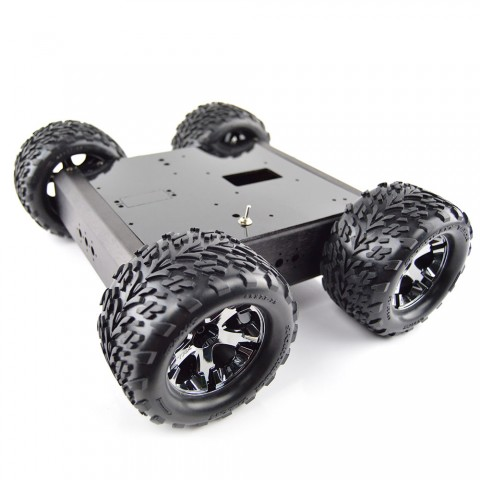
\includegraphics[width=0.25\textwidth]{lynxmotion-aluminum-a4wd1-rover-kit-w-encoders-7}
\end{wrapfigure}

The mobile base used is the Lynxmotion A4WD1 Rover, shown on the right. This kit comes with four 200 rpm dc gear motors, and four optical quadrature motor encoders.

\begin{wrapfigure}{l}{0.25\textwidth}
	\caption{Sabertooth 2x12 \cite{fig_sabertooth}}
	\centering
	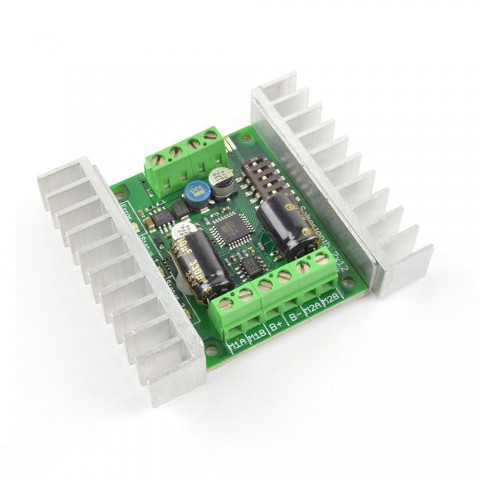
\includegraphics[width=0.25\textwidth]{sabertooth-dual-regenerative-motor-driver_3}
\end{wrapfigure}

The motors are controlled by a Sabertooth dual-channel 12A 6V-24V regenerative motor driver, shown on the left. This motor driver is powered by two LG 18650 HE2 rechargable lithium ion cells, which sit in an 18650 battery case which has been soldered to act as a battery pack with two 18650 cells in series. The battery cells are individually charged before use with a NiteCore-i2-V2014 li-ion charger.

\begin{wrapfigure}{r}{0.25\textwidth} %this figure will be at the right
	\caption{PING))) Ultrasonic Sensor \cite{fig_ping}}
	\centering
	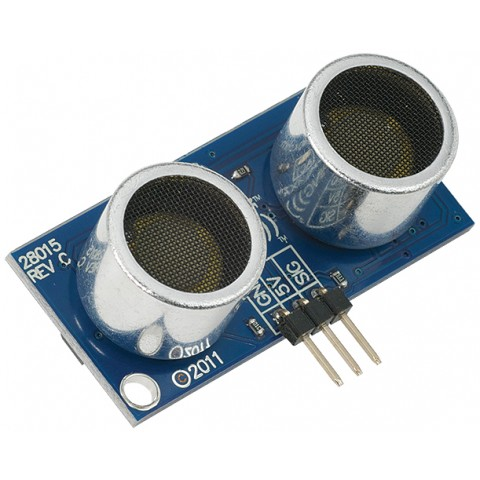
\includegraphics[width=0.25\textwidth]{parallax-ping-ultrasonic-sensor_1}
\end{wrapfigure}

On top of the rover is the PING))) ultrasonic distance sensor, which is attached to a standard Parallax servo which pans back and forth 180 degrees.

\begin{wrapfigure}{l}{0.25\textwidth}
	\caption{Arduino Uno R3 \cite{fig_arduino_uno}}
	\centering
	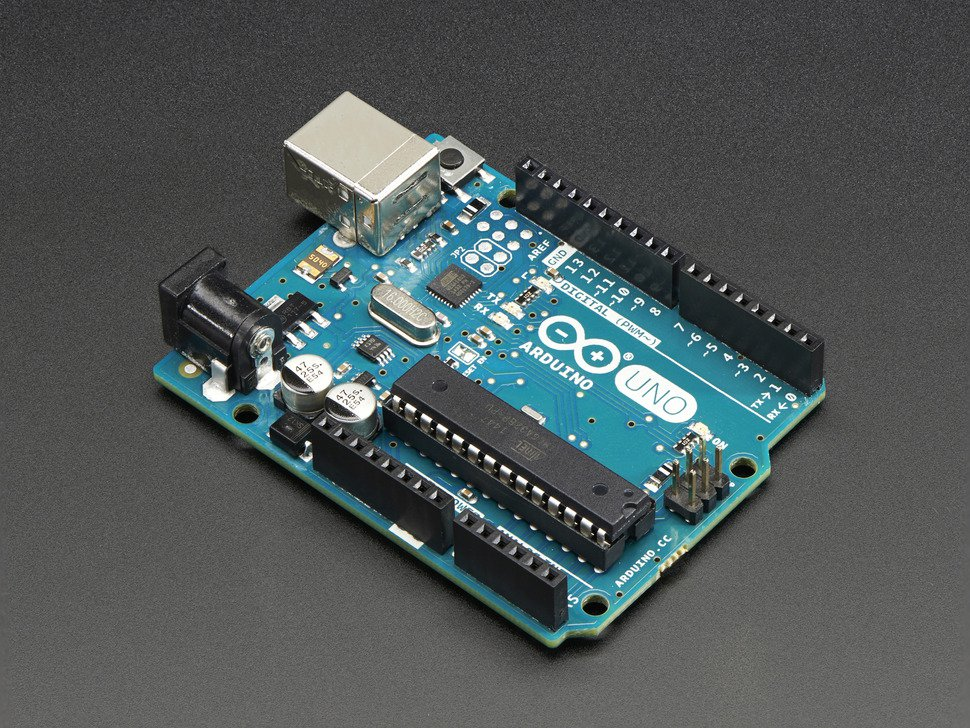
\includegraphics[width=0.25\textwidth]{arduinoUno}
\end{wrapfigure}

At the center of the rover is an Arduino Uno R3. This microcontroller handles several important tasks. It tells the motor driver what speed to set its two output channels to, and directly controls the panning motion of the standard Parallax servo. It also acts as a go-between for the digital output of the sensors on the rover and a laptop. It's connected to this laptop via a USB cable, which powers the board and allows communication over a serial port. Motor encoder values and ultrasonic range data are transmitted to the laptop, and motor power commands are received.

The specific laptop used in this project is the Dell Inspiron 3531, which has a quad core 2.16 GHz processor, and 4 GB of RAM. While these are relatively limited computational resources, the laptop was a personal work machine and already available to use for no additional cost. The machine is used as the main processing unit for the navigation logic. 

The last component is a Nexus 4 smartphone placed on the top panel of the rover, which is also connected to the laptop by USB. Inside this phone is an MPU-6050 chip which contains a gyroscope and accelerometer. Elsewhere on the phone's logic board are a magnetometer, otherwise known as a digital compass, and a GPS receiver. This smartphone was also already available, and acts as a cheap Inertial Measurement Unit (IMU) and GPS receiver for the robot.

\section{Construction}

\begin{figure}[h]
	\caption{Connections Made}
	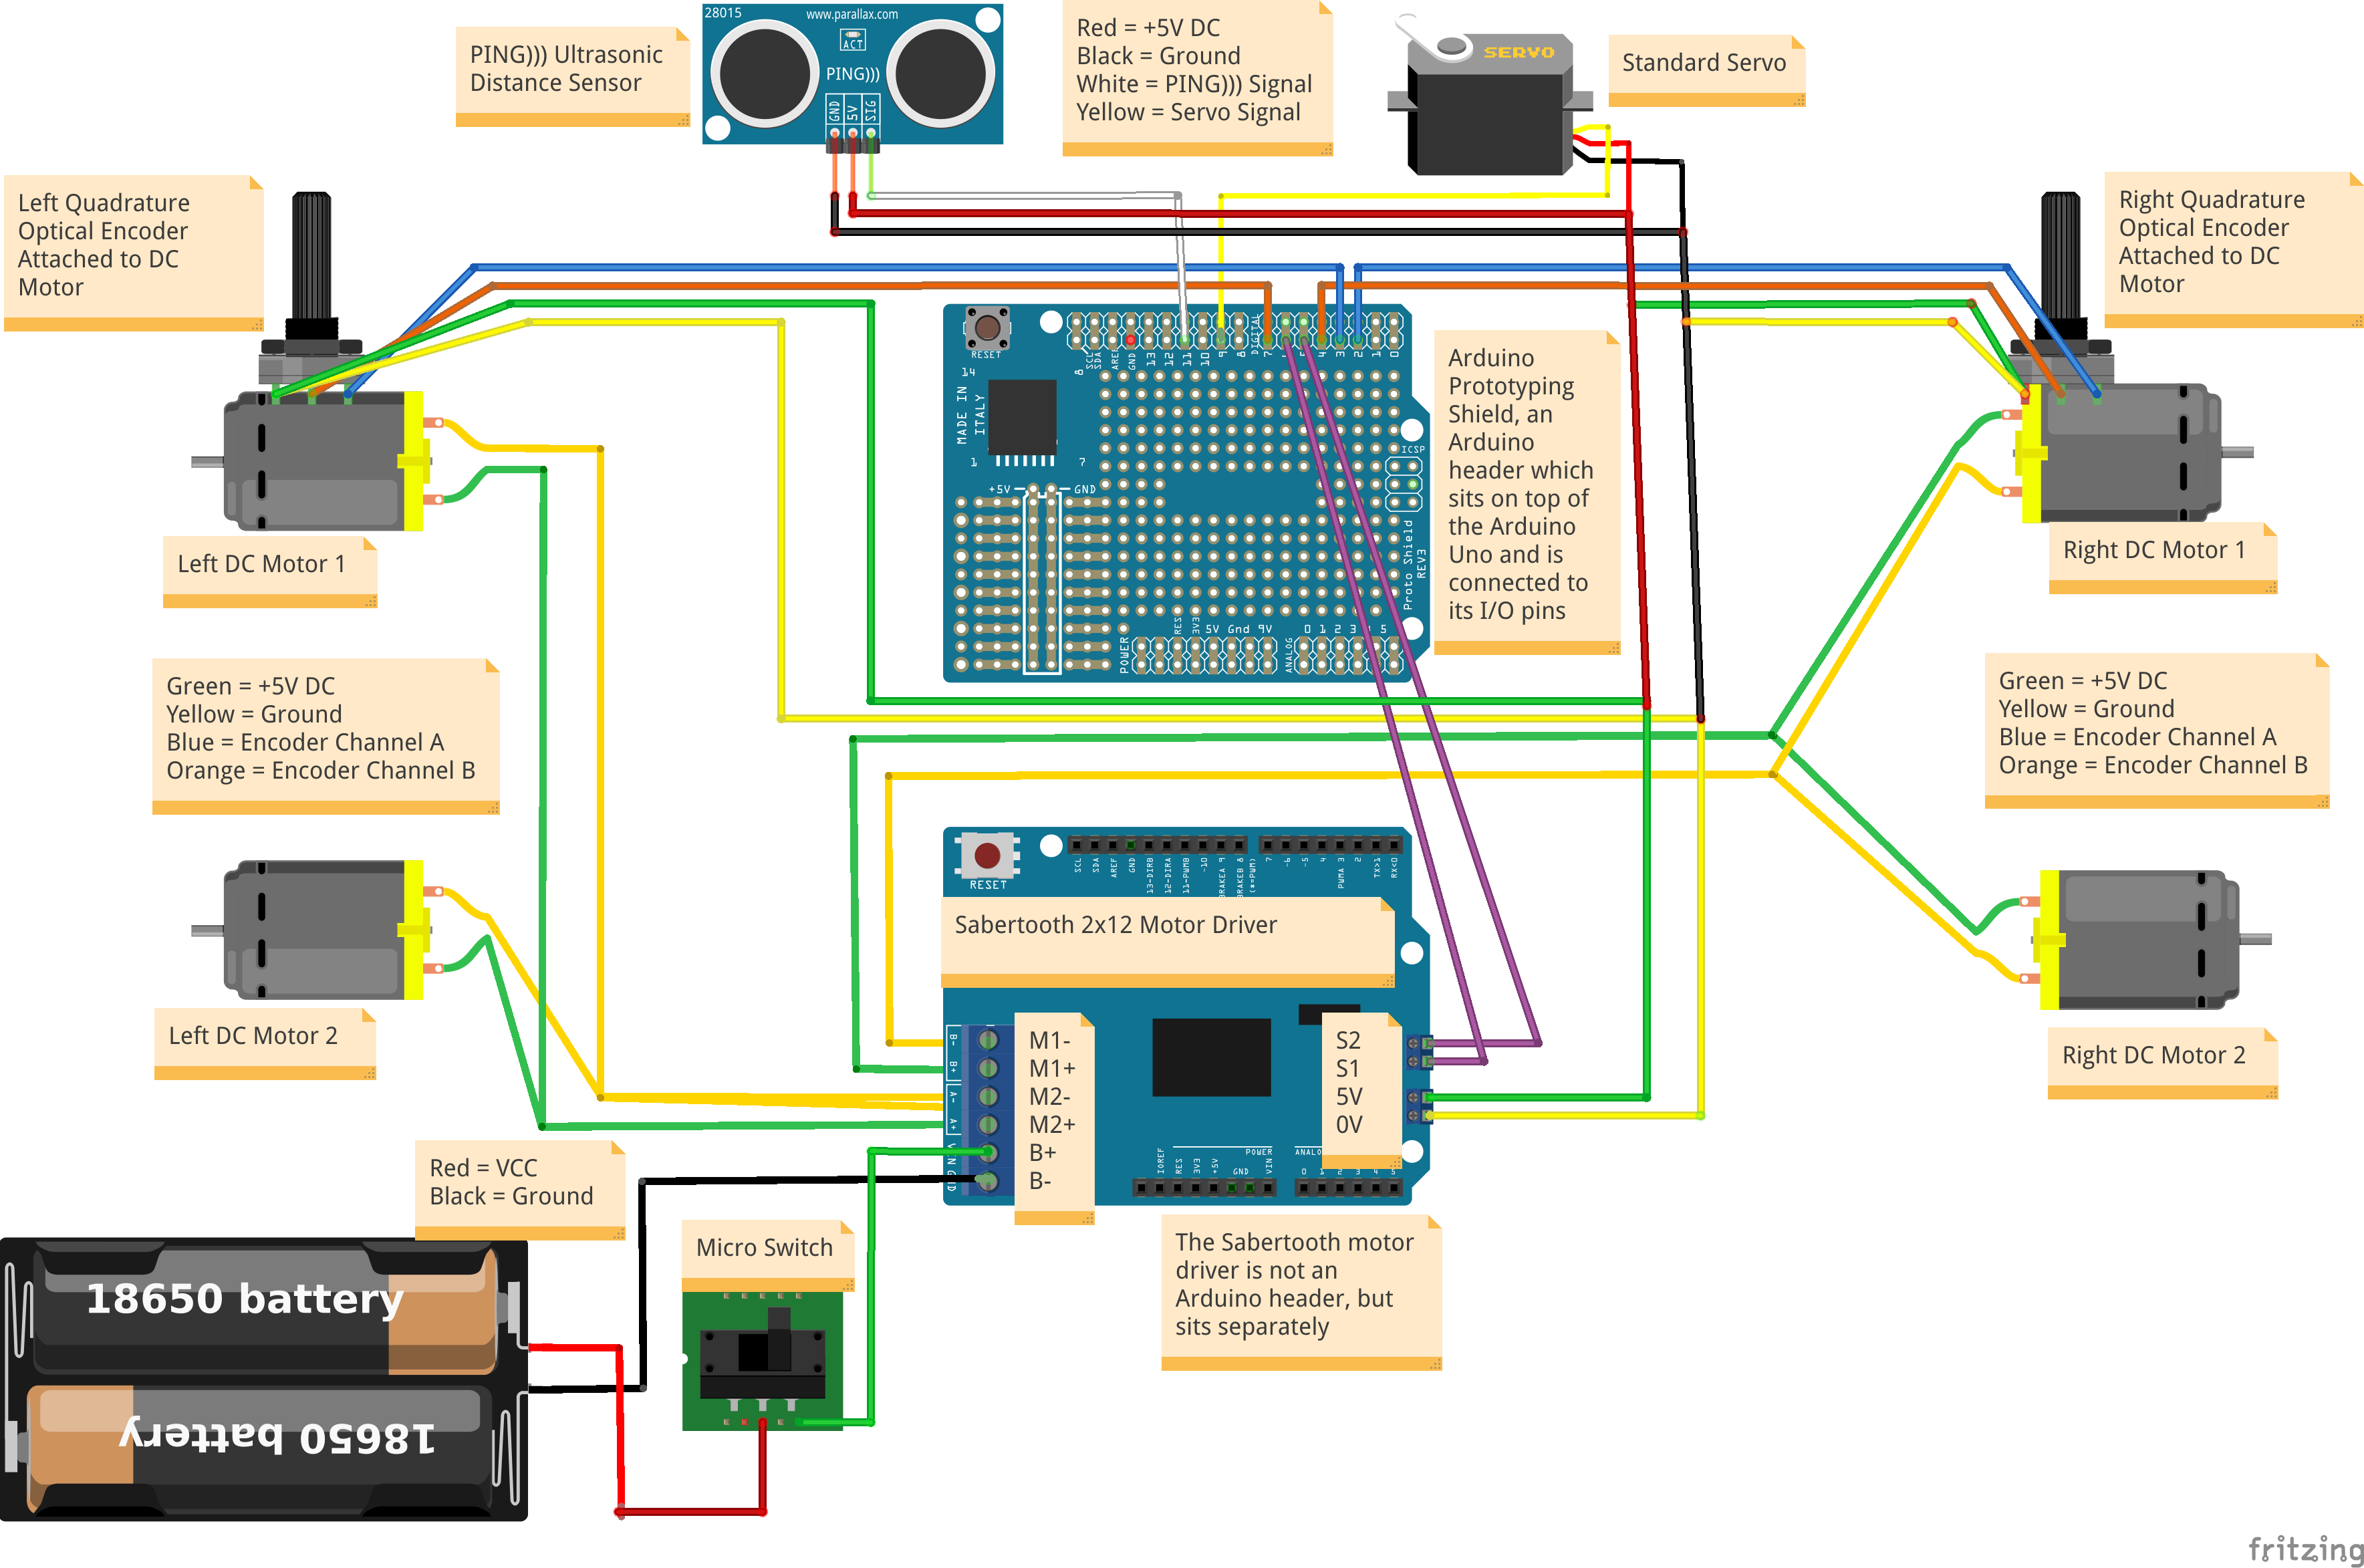
\includegraphics[width=\textwidth,height=\textheight,keepaspectratio]{RoverDesign}
	\centering
	\text{This image was created with Fritzing.}
\end{figure}

\subsection{Arduino Pin Connections}
Most digital pin numbers used are arbitrary, and connections may be permuted without any change. The sole exception  for Special care is taken in the 

\section{Arduino Sketch}
A sketch is Arduino-speak for a program uploaded to the board which will run on a loop as long as the board is powered.

\chapter{Arduino}

%BRIDGE FROM PREVIOUS SECTION
The Arduino Uno in this project acts as a bridge between hardware and software, allowing the the laptop to read sensor data from the rover, and control the speed of its wheels.

\section{Background}
Arduino development boards are printed circuit boards capable of running small embedded programs. They contain an on-board microcontroller, timing crystal, USB port, I/O pins and more. The specific board used in this project, an Arduino Uno, uses the ATmega328P microcontroller with a 16 MHz quartz timing crystal and 14 digital I/O pins. It also has 6 analog-to-digital converter I/O pins, but we won't make use of them in this project. 

Digital I/O pins can be configured to either read signals as input or generate them as output. Digital pins read input signals at specific times as binary values, i.e. the connected signal's voltage is read as either on or off compared to a certain threshold voltage. Following the standard Arduino literature, we will refer to these signals as either HIGH or LOW. When digital pins are configured to generate HIGH or LOW signals, they produce a relative output voltage above or below the threshold voltage.

\subsection{Servo Control Pulses} \label{sectionRCPulses}
An important use-case which pops up often when using the Arduino is that of interfacing with RC electronics. In this project's design, both the Sabertooth motor driver and the standard servo require their signal inputs to use the standard R/C transmission protocol.

This protocol involves sending brief HIGH pulses of variable width, between one and two milliseconds. There is a fixed delay between pulses, commonly about 20 ms of LOW signal. The width of the HIGH pulse communicates to a servo the desired position. Its internal components then drive its DC motors until the servo is rotated to the commanded position. In the case of the Sabertooth motor driver, the position is interpreted as a speed to drive the motors at.

\section{Arduino Uno Connections}
Refer back to Figure \ref{figRoverDesign} for a visual representation of how the Arduino Uno is connected to the other rover components.

\subsection{Hardware Interrupt Pins} \label{sectionHIP}
As one can see in Figure \ref{figRoverDesign}, only two optical quadrature encoders are used, placed on the front motors on the left and right side of the rover. This is due to a hardware limitation of the Arduino Uno. The ATmega328P microcontroller has only two interrupt pins, which are mapped to digital pins 2 and 3 on the Uno. These pins can trigger unique Interrupt Service Routines (ISRs) whenever the input signals change from LOW to HIGH voltage, or vice versa.

While it is possible to react to a change in any digital pin's voltage, it would be significantly slower than a hardware interrupt. An ISR is necessary to keep up with the fast rate of pin voltage changes that occur in the output of quadrature encoders.

If a different Arduino board such as the Mega were used, there would be sufficient hardware interrupt pins for all four encoders. Using a board with plentiful interrupts, one could even attach both channel outputs of the encoders to interrupt pins, rather than only one. This would double the encoders' resolution. See section \ref{sectionQuadEncoders} for more detail.

\subsection{Digital Pin Connections}
Each motor encoder has two output channels, A and B. Both encoders attach one of their output channels, channel A, to a hardware interrupt pin. In section \ref{sectionQuadEncoders} we will see why this configuration was chosen. The right motor's encoder connects channel A to pin 2, and channel B to pin 4. The left motor's encoder connects its channel A output to pin 3, and its channel B output to pin 7.

The S1 and S2 signal input terminals on the Sabertooth motor driver are connected to digital pins 5 and 6. The control signal for the hobby servo is connected to digital pin 9. The signal pin on the ultrasonic sensor is connected to digital pin 11. The Arduino's ground pin is connected to the ground of the motor driver's BEC, to ensure a common ground plane.

Most digital pin numbers used are arbitrary, and connections may be permuted without issue. The exceptions are pins 0-3, which must not be modified. Pins 0 and 1 must be left unattached for serial data transfer to work properly over USB. And pins 2 and 3 are hardware interrupt pins which must be used to handle the quadrature encoders' output.

\section{Motor Driver's Configuration}
The Sabertooth motor driver has two signal input terminals, S1 and S2, which allow the Arduino to issue instructions specifying how to drive the motors. The protocols used to communicate with the motor driver over these signal inputs are specified by six DIP switches on-board the driver. These DIP switches are manually flipped either up or down.

Setting switch 1 down and switch 2 up places the driver into R/C input mode, which configures S1 and S2 to expect servo control pulses, à la R/C controllers. This protocol was briefly explained in section \ref{sectionRCPulses}. \cite{sabertoothUserGuide}

Turning switch 3 down selects the lithium cutoff mode, which detects the number of lithium cells in series powering the driver, and shuts off when the battery pack's voltage drops below 3.0V per cell, or 6.0V for the two cell battery pack this project uses. This prevents accidental damage to the 18650 cells which may be caused by over-discharge.

Flipping switch 4 down selects independent (differential) drive, which allows S1 and S2 to each independently control the speed of one motor channel. Using this mode, turning of the vehicle is achieved by lowering the relative speed of the motors on one side of the vehicle compared to the other.

Switch 5 is flipped up to ensure a linear rather than exponential response of the motors to the Arduino's input signal. Switch 6 is flipped down to select "microcontroller mode", which turns off auto-calibration of the zero-velocity input signal, and turns off an automatic timeout. Thus if the signal connection is somehow lost the motor driver will continue driving the motors according to the last signal received. This is necessary for smooth performance of the motors since the Arduino may slightly delay control pulses. Though this introduces a risk of loss of control should wires come disconnected, it is a small one that should only occur during a catastrophic crash.

\section{Arduino Sketch}
A sketch is Arduino-speak for an embedded program written for an Arduino board. There is an Arduino IDE which supports development of sketches in C or C++, and allows one to take advantage of a software library for common I/O interactions. After the code is written in this IDE, it is uploaded to the board over a USB serial connection. The board will then continuously execute the code found in the sketch's main loop as long as the board is powered. This embedded software interacts with the various sensors and other electronics on a low level, through reading from and writing to the Arduino's digital I/O pins.

One of the standard Arduino libraries is the Servo library. This library allows one to configure a digital pin to output RC control pulses, as explained in section \ref{sectionRCPulses}. The sketch used in this project uses this library to specify the speed of each set of wheels driven by the Sabertooth motor driver, and to control the position of the standard servo aiming the ultrasonic range sensor. The motor driver is sent pulses every 20 ms, with HIGH pulses from 1 ms to 2 ms. The standard servo is also sent pulses every 20 ms, with HIGH pulses from 0.75 ms to 2.25 ms as its datasheet specifies.

\subsection{Ultrasonic Sensor}
The PING))) ultrasonic distance sensor works by emitting a short burst of 40 kHz sound waves and timing the delay before an echo response. The Arduino triggers a ping by generating a brief 5 \(\mu\)s (microsecond) pulse on the sensor's bi-directional signal pin. The sensor then generates a HIGH output pulse, which continues until either the echo is received or the maximum amount of time, 18.5 ms, has passed. This time may then be multiplied by the speed of sound in air to calculate an estimated distance of the first object in front of the sensor. \cite{pingDocumentation}

The sketch uses the NewPing library to handle this protocol \cite{newPing}. This library provides a convenient method, ping() which returns the echo time in \(\mu\)s. The sketch avoids costly floating point computations by sending this echo time over serial rather than a distance.

\subsection{Servo}
The ultrasonic sensor can only detect objects which are roughly straight in front of it. Thus for the rover to have a better approximation of its surroundings, the sensor needs to be panned back and forth. This is what the standard servo it is attached to allows. The sketch makes use of the Servo library to control the servo with R/C pulses. An angular degree from 0 to 180 is written to a Servo object, and the Servo library handles generating the output signal corresponding to that position on the appropriate digital pin.

The sketch sweeps the servo back and forth one degree at a time, and at each step an ultrasonic ping is emitted. The echo time for that ping is measured, and the current values of all sensors are published. This means that the delay between servo steps defines the publishing frequency of sensor data on the Arduino. This delay is currently set to 100 ms, which corresponds to a 10 Hz publishing frequency. The frequency could be increased for future work, but a bare minimum delay of 30 ms is necessary to give the servo time to finish moving, and the PING))) sensor time to recover and prepare for the next ping.

The basic idea is shown in the following code for an arbitrary servo step size:
\begin{mdframed}[backgroundcolor=light-gray, roundcorner=10pt,leftmargin=1, rightmargin=1, innerleftmargin=15, innertopmargin=15,innerbottommargin=15, outerlinewidth=1, linecolor=light-gray]
	\begin{lstlisting}[language=C++]
	while (servoPos < SERVO_LEFT) {
	sonicServo.write(servoPos); // Set servo position
	timer = millis(); // current time in ms
	while (millis() - timer <  SERVO_STEP_DELAY) {
	nh.spinOnce(); // handle callbacks
	}
	ping_time_uS = sonar.ping(); // Get echo time
	publishSensorMessages(servoPos, ping_time_uS);
	servoPos += SERVO_STEP_SZ;
	}
	\end{lstlisting}
\end{mdframed}

This code fragment is run inside the sketch's main loop, with a similar while-loop running right after, decrementing the servo position back to SERVO\_RIGHT.

millis() is an Arduino built-in function which uses a hardware timer to count how many milliseconds have passed since the board was turned on. The callback handling that occurs while waiting reads the incoming serial buffer for any data, and if motor commands are found, an appropriate callback function is executed. publishSensorMessages() sends over serial the ping echo time, the servo's current angle, and the tick counts of both encoders. Section \ref{sectionRosSerial} will further describe how this data is passed between laptop and Arduino.

\subsection{Quadrature Encoders} \label{sectionQuadEncoders}
An important function of the Arduino sketch is to track the movement of the motors. Our system may command the motor driver to move the rover's wheels with a certain fraction of the maximum available power, but it is difficult to predict with precision the resulting angular velocity. For one thing, the RPM of DC motors is proportional to the supplied voltage. But the voltage supplied to the motors through the motor driver is coming from an external li-po battery pack, which generates variable voltage. It starts at 8.4V and drops to a minimum of 6.0V before the motor driver shuts off. Thus even if the same servo control pulse is continuously sent to the motor driver, the motors' angular velocity will decrease over time.

In order to determine the true angular velocity of the motors, rotary encoders are attached to them. These feedback devices are incremental position encoders, meaning they monitor the change in the motor shaft's position compared to some starting position. 

\begin{wrapfigure}{l}{0.5\textwidth}
	\caption{\cite{fig_optical_encoders}}
	\centering
	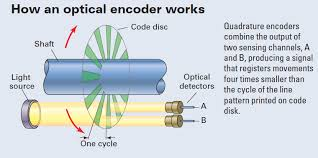
\includegraphics[width=0.5\textwidth]{opticalEncoders}
	\label{FigOpticalEncoders}
\end{wrapfigure}

The motor encoders which came with the Lynxmotion rover kit are optical quadrature encoders. This type of encoder attaches a flat disk with thin slits known as the code disk to the motor's gear shaft. Two photodiodes, components which transform light into electric current, are placed above the disk side by side. A light source shines light through the disk from the other side. See Figure \ref{FigOpticalEncoders} for a visual illustration.

As the motor spins the gear shaft, the code disk turns with it. This produces an on-off pattern of light on the photodiodes, which produce two square waves as signal outputs. These two channels of output pulses are referred to as channels A and B. Depending on the direction of rotation, channel A's square wave will either lag behind or be ahead of channel B. This can be seen in Figure \ref{FigQuadChannels} which shows example output pulses as a motor turns clockwise (CW) or counter-clockwise (CCW). \cite{encoderBlog}

The number of slits in the code disk corresponds directly to how many pulses each channel will produce in one revolution of the DC motor. This is known as the pulses per revolution (PPR), and is given by the manufacturer. By counting how many pulses occur in one second, and using the PPR, one can calculate the angular speed of the motor. If one wishes for greater resolution, they can watch each square wave for a change in voltage from LOW to HIGH or HIGH to LOW. This gives a maximum resolution of \(4 * PPR\) detectable position increments per revolution.

\begin{figure}[h]
	\caption{\cite{fig_quad_channels}}
	\centering
	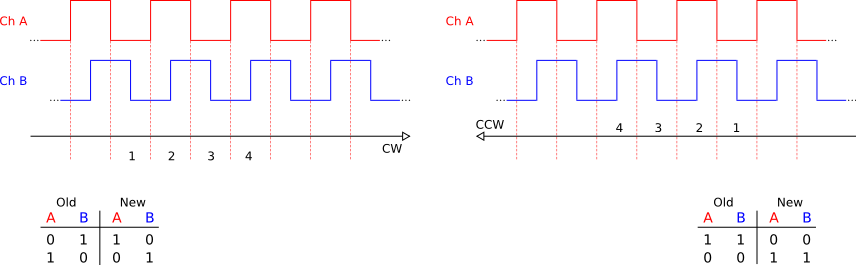
\includegraphics[width=\textwidth]{quadrature}
	\label{FigQuadChannels}
\end{figure}

Handling rapid changes in voltage is exactly what hardware interrupts are designed for. Unfortunately, for maximum resolution each encoder needs two hardware interrupt pins, one for each channel. The Arduino Uno only has two hardware interrupt pins, and our rover has two sides. It would be nice if we could at least use two encoders, one for each side.

We achieve this by reacting to changes in voltage in only one channel per encoder. In the two tables in Figure \ref{FigQuadChannels}, LOW voltage values are encoded as 0, and HIGH voltage values as 1. The first plot in the figure shows the output of the two channels when the motor is moving in the CW direction.  When channel A transitions from the section labeled 1 to section 2, it is rising from 0 to 1, and channel B has value 0. That information alone tells us that the motor's gear shaft is turning, but not in what direction. However, at the next transition between sections 2 and 3, channel A falls from 1 to 0, and channel B has value 1. Now we are confident that channel B began its pulse after channel A. This means that the photodiode generating channel B detected light after channel A's photodiode, i.e. the code disk is turning in the direction of photodiode A to B. Datasheet specifications will tell us that this translates to the CW direction. It turns out that for each channel A transition event, the previous and new channel values are sufficient to uniquely determine the direction of rotation of the motor. Thus, while only monitoring one of the channels lowers our resolution to \(2 * PPR\) counts per revolution, it allows us to use hardware interrupts for two quadrature encoders rather than only one. \cite{encoderBlog}

The sketch uses an implementation described in \cite{encoderBlog}, which creates a lookup table using the four binary digits representing the previous and current channel states. These digits form a four-bit binary number, which indexes into a sixteen element array. Each element of this array stores either 1, -1, or 0, where 1 represents a movement in the CW direction, -1 represents a movement in the CCW direction, and 0 represents an indeterminate transition. This lookup table is then used by the sketch when it reacts to a hardware interrupt caused by the channel A output of one of the encoders. When this interrupt occurs, the code reads the values of channels A and B from the corresponding digital pins, and combines them with the previous values to find the appropriate index in the lookup table. The value at that index is then added to a global counter variable, which keeps track of the net number of incremental movements from the motor's starting position. A net negative number indicates how far the motor has rotated in the CCW direction since it started, and a net positive number indicates how far the motor has rotated in the CW direction. \cite{encoderBlog}

The implementation described above is shown in the following C code of the ISR for the left encoder. \cite{encoderBlog}
\begin{mdframed}[backgroundcolor=light-gray, roundcorner=10pt,leftmargin=1, rightmargin=1, innerleftmargin=15, innertopmargin=15,innerbottommargin=15, outerlinewidth=1, linecolor=light-gray]
	\begin{lstlisting}[language=C++]
	volatile long encLeftCount = 0L;
	const int8_t encoder_lookup_table[] =
	{0,0,0,-1,0,0,1,0,0,1,0,0,-1,0,0,0};
	void encoderLeft_isr() {
	static uint8_t encLeft_val = 0;
	encLeft_val = encLeft_val << 2;
	encLeft_val = encLeft_val |
	  ( ((PIND & 0b100) >> 1) | 
	  ((PIND & 0b10000) >> 4) );
	encLeftCount = encLeftCount +
	  encoder_lookup_table[encLeft_val & 0b1111];
	}
	\end{lstlisting}
\end{mdframed}

When the digital pin connected to the left encoder's Channel A output changes, the main loop of the sketch is interrupted, and this ISR is executed. Until this ISR finishes, no other code is run, including other ISRs, though they may be flagged for future execution. Therefore ISRs must be as fast as possible, to not cause any interrupt events to be dropped, and to ensure that the main loop continues running smoothly.

To this end, this ISR makes use of constants and low-level C and avr microcontroller commands to ensure a speedy execution, at the price of readability. PIND is an avr command which returns input readings from digital pins 0-7 encoded into a byte. Bit shifting and masking are then used to extract and store the values of pins 2 (channel A) and 4 (channel B) into the two least significant bits of the encLeft\_val variable. This variable is static, and so retains its value between ISR executions. The count is then incremented according to the lookup table.

When the sketch's main loop publishes sensor readings, it needs to publish the current encoder tick count for the right and left encoders. However, reading from multi-byte variables which are accessed within and without an ISR risks data corruption in the event that the ISR interrupts the main thread in-between readings of bytes. Since the encoder tick count variables are four bytes long, interrupt guards must be used around a read to make it atomic. These guards temporarily stop the custom ISR from executing while the global variables are copied over to local ones. This is shown for the left encoder count in the following snippet from the sketch:
\begin{mdframed}[backgroundcolor=light-gray, roundcorner=10pt,leftmargin=1, rightmargin=1, innerleftmargin=15, innertopmargin=15,innerbottommargin=15, outerlinewidth=1, linecolor=light-gray]
	\begin{lstlisting}[language=C++]
	detachInterrupt(digitalPinToInterrupt(encLeftAPin));
	encMsg.leftTicks = encLeftCount;
	attachInterrupt(digitalPinToInterrupt(encLeftAPin),
	  encoderLeft_isr, CHANGE);
	t = 0;
	\end{lstlisting}
\end{mdframed}

Similar guards are used for the right encoder count variable. 

Because we are turning interrupts off briefly, there is the risk that we could miss an interrupt event on one of the channel A pins. Missing an edge pulse from one of the encoders would not only lose that tick, but would also throw off the next value we index into the lookup table. Luckily, the Arduino has a single-bit interrupt event flag for every interrupt event. Therefore in the worst case scenario, an encoder interrupt event occurs just after the ISR handler is detached, and that event is flagged. As long as the ISR is reattached and handles that flag before a second interrupt event occurs, there won't be a problem. After reattaching the ISR, the next program instruction is guaranteed to be executed before handling any flagged events. To ensure speedy handling of a flagged event, a meaningless assignment of zero is made to the local variable t.

Let's calculate how often each interrupt event occurs. Each encoder generates 100 pulses per revolution. We will only be watching one of the square waves (output channel A), so that's 200 edge transitions per revolution. The motors are rated for 200 rpm, so at maximum speed the two encoders would revolve less than 3.4 times per second. So there will be at most \[3.4\ rev/sec * 200\ events/rev = 680\ events/sec\]
Meaning we are guaranteed to have at least \(1 / 680 \approx 1.4\ ms\) between encoder interrupt events.

So the interrupt guards need to take significantly less than \(1.4\ ms\) in order to allow a flagged interrupt event to be handled before the next event occurs. Each global encoder count variable is four bytes, so assignment compiles to four machine instructions. The assignment of zero to the one-byte variable t takes one machine instruction. The helper macro digitalPinToInterrupt() is a preprocessor \#define, and so takes zero machine instructions. Therefore there are five total machine instructions executed before the ISR is executed. The Arduino Uno uses a 16 MHz quartz timing crystal, so executing one instruction takes \[1 / (16000000\ Hz) = 0.000000625\ seconds = 62.5\ nanoseconds\]

Thus to run the five instructions takes \(5 * 62.5\ ns = 0.3125\ \mu s\). Then the flagged event must be handled. External interrupt calling has an overhead of 5.125 \(\mu s\), to enter and leave the function \cite{gammonInterrupts}. Thus as long as the ISR executes in less than \(1.4\ ms - 0.0003125\ ms - 0.005125\ ms = 1.3945625\ ms\), the sketch will never miss an encoder event. Testing of the ISR indicates that this is an order of magnitude more time than needed.
\chapter{ROS}

\section{ROS}
The Robot Operating System (ROS)


\subsection{Nodes}

\subsection{Frames}

\subsection{Topics}
publishing and subscribing messages


\section{Overview}

\section{Ros Sensors App}
Android app to publish IMU and GPS data from a smartphone.
\subsection{How to use}


\section{robot\_localization package}
odometry estimate from wheel encoders
\chapter{Field Test}

In order to test the rover's ability to localize itself, a simple field test was conducted in a parking lot. Inspiration for this experiment comes from Moore and Stouch \cite{robot_localization_paper}.

\section{Experiment Design}

The rover was initially placed in a parking lot oriented facing west. It was then driven in a roughly rectangular shape around the lot using the virtual\_joystick node, described in section \ref{sectionJoystick}. During this time the raw sensor data streaming in from the Arduino and phone was recorded and saved into a ROS bag file. The rover was driven in a loop, such that its initial and ending position and orientation were roughly equal. Total collection time was five and a half minutes.

See Figure \ref{fig:roverPath} for two representations of the path taken. Figure \ref{figRouteMemory} displays the path actually traversed, while Figure \ref{figRouteGPS} is constructed from the phone's GPS readings. At no point did the rover go onto the grass.

The ROS \textit{rosbag} utility was then used to repeatedly simulate the recorded sensor messages, while the EKF was run in different configurations. The rover's state was computed from raw wheel odometry, from wheel odometry fused with the IMU data, and from wheel odometry, IMU data, and GPS fixes all fused together. Refer to Table \ref{tab:configs} for a review of which state variables each sensor affects.

\section{Results}

% laptop had no problem computing using the filter. No memory spikes either. Very computationally efficient! laptop is enough for localization - is it enough for navigation?

During each filter computation, a state estimate was produced at 30 Hz in a local frame, and that output was then transformed into a global frame, where position is given as latitude and longitude. These gps coordinates were then plotted using the handy GPS Visualizer tool \cite{gps_visualizer}. Figure \ref{fig:ekfOutputs} displays those plots.

Figure \ref{figRouteOdom} shows the estimated path when fusing only the wheel encoder output. The initial upward trajectory and left turn are tracked reasonably well, but the second left turn rotates too far and throws the rest of the estimate off.

Figure \ref{figRouteOdomImu} shows the path generated when fusing wheel odometry with IMU data. In this case the shape of the path is much closer to truth, though the initial right turn is under-estimated.

Lastly, Figure \ref{figRouteOdomImuGps} shows the result of fusing both previous sensors with GPS fixes. This plot looks much like the raw gps plot in Figure \ref{figRouteGPS}, however upon close inspection one can see jagged jumps in position. These jumps are instantaneous and actually lead to a discontinuous position estimate, though the visualizing tool connects every point. They are caused by the filter instantaneously adjusting the position estimate based on an incoming gps fix. The filter does give weight to the current estimate, so the new adjusted position lies in between the gps fix and the old position estimate. Due to the frequent gps fixes and slow velocity of the rover, the estimated path does not vary too far from the raw gps path.

\begin{table}[h]
	\caption {Errors for Different Sensor Fusions \cite{robot_localization_paper}} \label{tab:errors} 
	\begin{center}
		\begin{tabular}{|c|c|c|} \hline
			\textbf{Sensors Fused} & \textbf{Loop Closure Error x,y (m)} & \textbf{Filter's Std. Dev. x,y (m)} \\ \hline
			Wheel Encoders & -88.37, -43.10 & 45.64, 126.36 \\ \hline
			Encoders + IMU & -12.90, -11.89 & 52.80,  52.02 \\ \hline
			Encoders + IMU + GPS & -0.97, -0.50 & 4.68,  4.56 \\ \hline
		\end{tabular}
	\end{center}
\end{table}

Table \ref{tab:errors} shows the position error between the rover's start and end positions for each filter configuration. Because the rover's local frame has its origin at the start point, this error is simply the last state estimate produced by the filter. The standard deviation for each dimension is also reported, giving an idea of the filter's confidence in its location. Note that the position errors are negative because the filter considers the end point to be behind and to the right of the rover's starting orientation, which puts it in the -X and -Y direction, according to ROS standards.

\begin{figure}[p] 
	\caption{
		The rover's path.
	}
	\label{fig:roverPath}
	\begin{subfigure}{\textwidth}
		\centering
		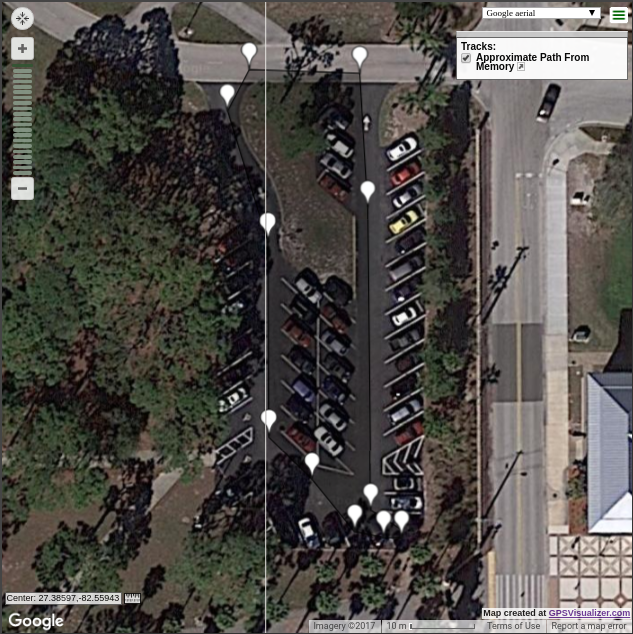
\includegraphics[height=0.45\textheight]{testRun/route_from_memory}
		\caption{Path Manually Mapped}
		\label{figRouteMemory}
	\end{subfigure}
	\begin{subfigure}{\textwidth}
		\centering
		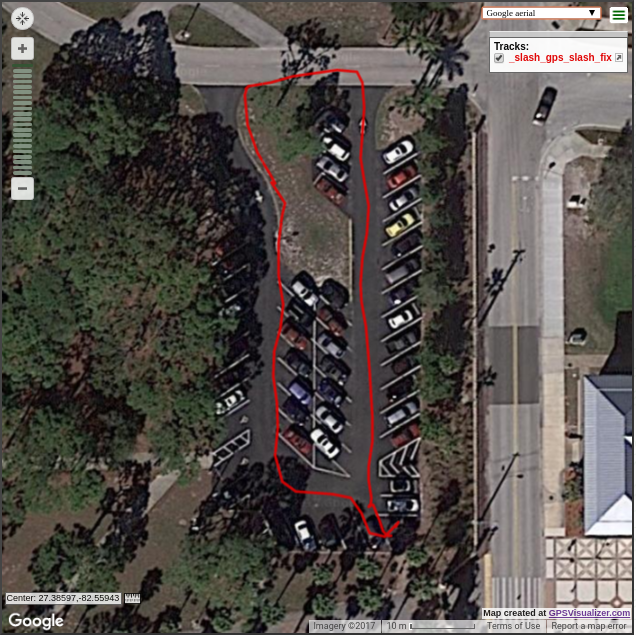
\includegraphics[height=0.4\textheight]{testRun/raw_gps_data}
		\caption{Path According to Phone's GPS}
		\label{figRouteGPS}
	\end{subfigure}
	
\end{figure}

\begin{figure}[p] 
	\caption{
		Filter Outputs For Different Sensor Fusions
	}
	\label{fig:ekfOutputs}
	\begin{subfigure}{\textwidth}
		\centering
		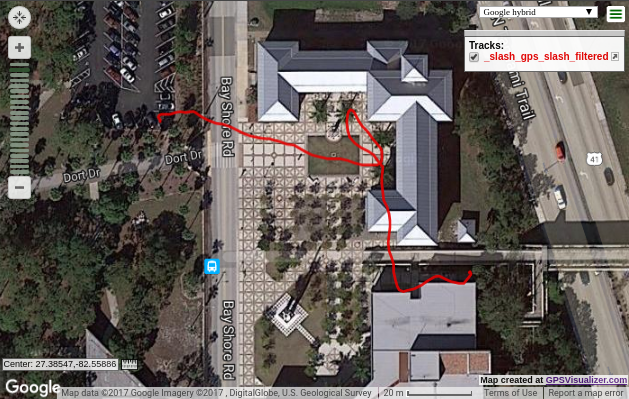
\includegraphics[height=0.4\textheight]{testRun/ekf_output_odom}
		\caption{Raw Wheel Odometry}
		\label{figRouteOdom}
	\end{subfigure}
	\begin{subfigure}{\textwidth}
		\centering
		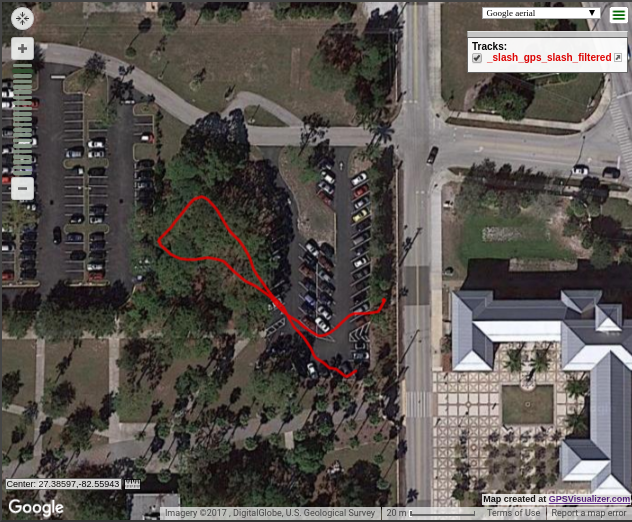
\includegraphics[height=0.4\textheight]{testRun/ekf_output_odom_imu}
		\caption{Wheel Odometry + IMU}
		\label{figRouteOdomImu}
	\end{subfigure}
	
\end{figure}

\begin{figure}[p] \ContinuedFloat
	\begin{subfigure}{\textwidth}
		\centering
		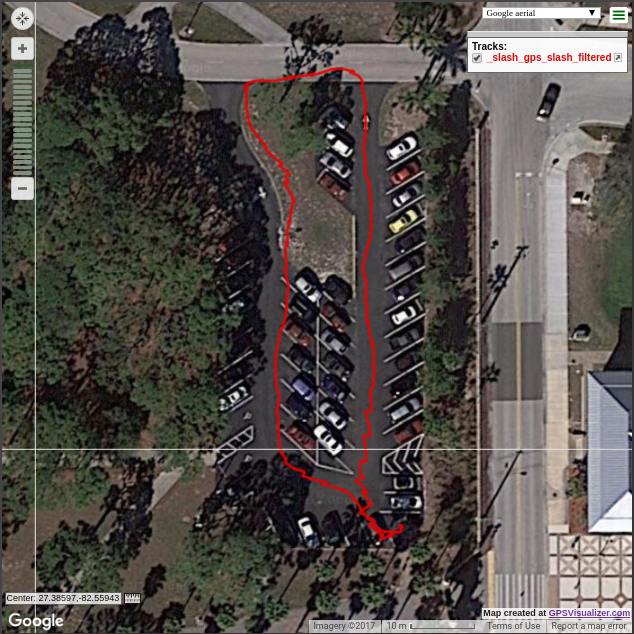
\includegraphics[width=\textwidth,height=\textheight,keepaspectratio]{testRun/ekf_output_odom_imu_gps}
		\caption{Wheel Odometry + IMU + GPS}
		\label{figRouteOdomImuGps}
	\end{subfigure}
\end{figure}
\chapter*{Conclusion}

We have shown that the proposed vehicle design is capable of using wheel encoders and a smartphone to localize itself with respect to UTM coordinates.

%Project Limitations
However, this localization is less precise than it could be, due to several flaws in the rover's design. The differential drive model is a simple approximation to the skid steering rover, causing large errors in the yaw state variable to accumulate quickly in the wheel odometry. The covariance matrices for the sensors are hard-coded rather than dynamically computed, and need to at least be empirically calibrated. And the magnetometer readings are affected by the magnetic field generated by the DC motors. This effect could be alleviated by adding a second level on top of the rover, putting more distance between the smartphone and motors.

%Original goal:
%Create a cheap outdoors autonomous robot. Given a 'map' of the New College campus, this robot should be able to navigate from one outdoors location to another using footpaths. In doing so, it should dynamically avoid obstacles such as people, and recalculate alternate routes when a route is unexpectedly blocked.

%Possible Extensions

It is hoped that this project is will be a jumping off point for future work. The logical next step would be to integrate the ultrasonic sensor's range and angle data into the project, as a slower approximation of LIDAR range data, which will allow the system to dynamically generate a map of the immediate area around the rover. Localization can then be performed in real-time with respect to this map.

%The most popular algorithm for global localization (i.e., localization including range data) is the adaptive Monte Carlo localization (amcl) system.


% not sure if this summary is accurate
%Amcl is another recursive Bayesian estimator based on Bayes Filter, which represents the state's belief distribution by a cloud of particles. Each particle represents a possible state, and each particle is assigned a probability weight based on the probability that the current sensor readings would be measured, given that that particle state was the true state. It uses random sampling to update its particle cloud over time.

%localization with respect to laser-based map landmarks 

%Range data would be fed into amcl, and it would adjust the 
%coming from the first EKF node which %outputs continuous local filtered odometry, 

%Its output would also be discontinuous, as recognition of a landmark previously seen will cause discrete jumps in amcl's position estimate.

Another possible extension would be to add video feed as a new source of sensor data, either via the laptop's webcam or the smartphone's built-in camera. The camera would need shock absorbers, or else the video frames would wobble. Perhaps video stabilization techniques could be used to compensate for this, in which case visual odometry could prove useful. The Arduino microcontroller board chosen in this design could be replaced with a larger model, or by a Raspberry Pi, which is a system on a chip that costs - at the time of this writing -roughly \$15 more than the Arduino board, but comes with additional features such as built-in WiFi and Bluetooth for short-range communication. 

On the software side, the differential\_drive package should eventually be replaced by the diff\_drive\_controller package, which performs the same function but integrates more naturally into the ROS navigation stack. The collection of software used in this project is available online at the following url: \url{https://github.com/NoahRJohnson/AutoRover}.

% gps and imu chip instead of phone, as far as software goes, mention the ROS navigation stack to facilitate actual autonomous navigation rather than just localization.

%Possible idea for simple navigation: GPS Waypoints. GPS markers form a linearized path travel in a straight line from one GPS node to another
% Could create waypoints using google maps, manually creating waypoints, and exporting to kml file, turning that into a csv file maybe?
%https://www.google.com/maps/d/edit?mid=1wKgTvF7i7Xdpi42cw1ffAOrGDVw&ll=27.38460862376806%2C-82.56151826455687&z=17



\addcontentsline{toc}{chapter}{Conclusion}
%\appendix
%\chapter{Tables}

\begin{table}
\caption{Armadillos}
\label{arm:table}
\begin{center}
\begin{tabular}{||l|l||}\hline
Armadillos & are \\\hline
our	   & friends \\\hline
\end{tabular}
\end{center}
\end{table}

\clearpage
\newpage

%\chapter{Figures}

\vspace*{-3in}

\begin{figure}
\vspace{2.4in}
\caption{Armadillo slaying lawyer.}
\label{arm:fig1}
\end{figure}
\clearpage
\newpage

\begin{figure}
\vspace{2.4in}
\caption{Armadillo eradicating national debt.}
\label{arm:fig2}
\end{figure}
\clearpage
\newpage

\addcontentsline{toc}{chapter}{Bibliography}
\printbibliography
\end{document}

